\documentclass[runningheads]{llncs}

\setlength{\paperheight}{232.8mm}
\setlength{\paperwidth}{151.5mm}
\setlength\voffset     {-23mm}
\setlength\hoffset     {-34mm}

%
\usepackage{hyperref}
\usepackage{multicol}
\usepackage[final]{changes}
\usepackage{url}
\usepackage{amsmath}
\usepackage{bm}
\usepackage{multirow}
\usepackage{tcolorbox}
\usepackage{rotating}
\usepackage{latexsym,amssymb,amsmath}
\usepackage{makecell}
\usepackage{xspace}
\usepackage{paralist}
\usepackage{wrapfig}
\usepackage{adjustbox}
\usepackage{cite}
%\usepackage{times}
%%%%%%%%%%%%%%%%%%%%%%%%%%%%%%%%%%%%%%%%%%%%%%%%%%%%%%%%%%%%%%%%%%%%%%%%%%%%%%
%%% Time-stamp: "2018-09-07 18:35:03 calvanese"
%%%%%%%%%%%%%%%%%%%%%%%%%%%%%%%%%%%%%%%%%%%%%%%%%%%%%%%%%%%%%%%%%%%%%%%%%%%%%%

%%%%%%%%%%%%%%%%%%%%%%%%%% General Math

\newcommand{\A}{\ensuremath{\mathcal{A}}}
\newcommand{\B}{\ensuremath{\mathcal{B}}}
%\newcommand{\C}{\ensuremath{\mathcal{C}}}
\newcommand{\D}{\ensuremath{\mathcal{D}}}
\newcommand{\E}{\ensuremath{\mathcal{E}}}
\newcommand{\F}{\ensuremath{\mathcal{F}}}
%\newcommand{\G}{\ensuremath{\mathcal{G}}}
\renewcommand{\H}{\ensuremath{\mathcal{H}}}
\newcommand{\I}{\ensuremath{\mathcal{I}}}
\newcommand{\J}{\ensuremath{\mathcal{J}}}
\newcommand{\K}{\ensuremath{\mathcal{K}}}
\renewcommand{\L}{\ensuremath{\mathcal{L}}}
\newcommand{\M}{\ensuremath{\mathcal{M}}}
\newcommand{\N}{\ensuremath{\mathcal{N}}}
\renewcommand{\O}{\ensuremath{\mathcal{O}}}
\renewcommand{\P}{\ensuremath{\mathcal{P}}}
\newcommand{\Q}{\ensuremath{\mathcal{Q}}}
\newcommand{\R}{\ensuremath{\mathcal{R}}}
%\renewcommand{\S}{\ensuremath{\mathcal{S}}}
\newcommand{\T}{\ensuremath{\mathcal{T}}}
%\newcommand{\U}{\ensuremath{\mathcal{U}}}
\newcommand{\V}{\ensuremath{\mathcal{V}}}
\newcommand{\W}{\ensuremath{\mathcal{W}}}
\newcommand{\X}{\ensuremath{\mathcal{X}}}
\newcommand{\Y}{\ensuremath{\mathcal{Y}}}
\newcommand{\Z}{\ensuremath{\mathcal{Z}}}

%%%%%%%%%%%%%%%%%%%%%%%%%% Abbreviations

%%\newcommand{\eset}{\emptyset}
%%\newcommand{\col}{\colon}
\newcommand{\ol}[1]{\overline{#1}}                % overline
%\newcommand{\ul}[1]{\underline{#1}}               % underline
%%\newcommand{\uls}[1]{\underline{\raisebox{0pt}[0pt][0.45ex]{}#1}}
%% ul with space between text and line

\newcommand{\ra}{\rightarrow}
\newcommand{\Ra}{\Rightarrow}
\newcommand{\la}{\leftarrow}
\newcommand{\La}{\Leftarrow}
%\newcommand{\lra}{\leftrightarrow}
\newcommand{\Lra}{\Leftrightarrow}
\newcommand{\lora}{\longrightarrow}
\newcommand{\Lora}{\Longrightarrow}
\newcommand{\lola}{\longleftarrow}
\newcommand{\Lola}{\Longleftarrow}
\newcommand{\lolra}{\longleftrightarrow}
\newcommand{\Lolra}{\Longleftrightarrow}
%\newcommand{\ua}{\uparrow}
\newcommand{\Ua}{\Uparrow}
\newcommand{\da}{\downarrow}
\newcommand{\Da}{\Downarrow}
\newcommand{\uda}{\updownarrow}
\newcommand{\Uda}{\Updownarrow}

%%%%%%%%%%%%%%%%%%%%%%%%%% Relations

%%\newcommand{\incl}{\subseteq}
%%\newcommand{\imp}{\rightarrow}
\newcommand{\per}{\mbox{\bf .}}                  % period

%%%%%%%%%%%%%%%%%%%%%%%%%% Delimiters

%%\newcommand{\quotes}[1]{{\lq\lq #1\rq\rq}}
%\newcommand{\set}[1]{\{#1\}}                      % set
%\newcommand{\Set}[1]{\left\{#1\right\}}
\newcommand{\bigset}[1]{\Bigl\{#1\Bigr\}}
\newcommand{\bigmid}{\Big|}
\newcommand{\size}[1]{|{#1}|}                     % cardinality of a set
%%\newcommand{\Card}[1]{\left| #1\right|}
\newcommand{\card}[1]{\sharp #1}
\newcommand{\tup}[1]{\langle #1\rangle}            % tuple
\newcommand{\Tup}[1]{\Braket{#1}}
\newcommand{\norm}[2]{\|#1\|_{#2}}
\newcommand{\setone}[2][1]{\set{#1\cld #2}}

%%%%%%%%%%%%%%%%%%%%%%%%%% STYLING AND SPACING

%\newcommand{\inlinetitle}[1]{\smallskip\noindent\textbf{#1.}\xspace}





\newcolumntype{C}{>{\centering\arraybackslash}X}

%\makeatletter
%\g@addto@macro\normalsize{%
%\setlength{\abovecaptionskip}{-2pt}
%\setlength{\belowcaptionskip}{12pt}
%\setlength\abovedisplayskip{3pt}
%\setlength\belowdisplayskip{3pt}
%\setlength\abovedisplayshortskip{3pt}
%\setlength\belowdisplayshortskip{3pt}
%}
%\makeatother

\newcounter{dummy} 
\newcounter{dummy1} 
\newcounter{dummy2}
\newcounter{dummy3} 
\newcounter{dummy4}
\newcounter{dummy5} 
\newcounter{dummy6}
\newcounter{dummy7}
%\numberwithin{dummy}{section}

\usepackage[thmmarks,amsmath]{ntheorem}
%\theorempreskip{1pt}
%\theorempostskip{1pt}

%\theoremstyle{plain}
%\theorembodyfont{\normalfont}
%\theoremseparator{.}
%\let\definition\relax
%\theoremsymbol{\ensuremath{\square}}
%\newtheorem{definition}{Definition}


\let\proposition\relax
\let\theorem\relax
\let\lemma\relax
\let\definition\relax
\theoremseparator{.}
\theorembodyfont{\itshape}
\theoremsymbol{$\triangleleft$}
\newtheorem{theorem}[dummy]{Theorem}
\newtheorem{lemma}[dummy1]{Lemma}
\newtheorem{definition}[dummy2]{Definition}
\newtheorem{proposition}[dummy3]{Proposition}

\let\remark\relax
\let\example\relax
%\let\example*\relax
\theorembodyfont{\normalfont}
\newtheorem{example}[dummy4]{Example}
\newtheorem{remark}[dummy5]{Remark}
%\newtheorem{example*}[dummy4]{Example}


\theoremstyle{nonumberplain}
\theoremheaderfont{\itshape}
\theorembodyfont{\normalfont}
\let\proof\relax
\theoremseparator{.}
\theoremsymbol{\ensuremath{\dashv}}
\newtheorem{proof}[dummy6]{Proof}


\qedsymbol{\ensuremath{\dashv}}


%%% Local Variables:
%%% mode: latex
%%% TeX-master: "main"
%%% save-place: t
%%% End:

\usepackage{todonotes}

\interfootnotelinepenalty=10000
\usepackage{graphicx}
\usepackage{xcolor,color}
\usepackage{subfig}
\usepackage{tikz}
\usepackage{calc}

\usepackage{tabularx}
\usepackage{booktabs}

\usepackage{ulem}

\usepackage{kbordermatrix}
\usepackage{amsmath,amsfonts}
\usepackage{braket}
\usepackage{xfrac}

\usepackage{pifont}
\usepackage{amssymb}
\usepackage{paralist}
\usepackage[inline]{enumitem}

\usepackage{varioref}
\newcommand{\pmin}{\rho}

\newcommand{\const}[1]{\mathsf{#1}}

\newcommand{\alphabet}{\Sigma}
\newcommand{\tasks}{\mathcal{A}}
\newcommand{\hidden}{\tau}

\newcommand{\uswn}{SWN\xspace}
\newcommand{\net}{\ensuremath{N}}
\newcommand{\tg}{\ensuremath{G}}
\newcommand{\closed}[1]{\overline{#1}}
\newcommand{\marking}{m}
\newcommand{\enaset}[2]{E_{#2}(#1)}
\newcommand{\fire}[4]{#1\xrightarrow{#2}_{#4}#3}
\newcommand{\probt}[3]{\mathbb{P}_{#2,#3}(#1)}
\newcommand{\prob}[2]{\mathbb{P}_{#2}(#1)}
\newcommand{\rg}[1]{RG(#1)}
\newcommand{\ind}[1]{\textnormal{\texttt{#1}}}
\newcommand{\seq}{\eta}
\newcommand{\run}{\xi}
\newcommand{\trace}{\sigma}
\newcommand{\traces}[1]{\mathit{traces}(#1)}
\newcommand{\ptraces}[2]{\mathit{ptraces}_{#2}(#1)}

\newcommand{\nreach}[3][]{#2 \overset{#1}{\rightsquigarrow} #3}
\newcommand{\runs}[2]{runs_{#2}(#1)}
\newcommand{\seqs}[2]{seqs_{#2}(#1)}
\newcommand{\transp}[1]{#1^\top}
\newcommand{\embed}{\phi}
\newcommand{\trembed}{\embed^{\text{tr}}}
\newcommand{\gorgembed}{\embed^{g}}


\newcommand{\pa}{\rho_{23}}
\newcommand{\pb}{\rho_{24}}
\newcommand{\pc}{\rho_{55}}
\newcommand{\pd}{\rho_{65}}
\newcommand{\pe}{\rho_{67}}
\newcommand{\pf}{\rho_{57}}

\newcommand{\logtrace}{\trace}
\newcommand{\nonlogtrace}{{\trace'}}


\newcommand{\approptoinn}[2]{\mathrel{\vcenter{
			\offinterlineskip\halign{\hfil$##$\cr
				#1\propto\cr\noalign{\kern2pt}#1\sim\cr\noalign{\kern-2pt}}}}}
\newcommand{\appropto}{\mathpalette\approptoinn\relax}


\newcommand{\unravelled}{unfolded}
\newcommand{\unravelling}{unfolding}
\newcommand{\unravel}{unfold}



%
%\def\WWITHN{def}
%\ifdefined\WWITHN
%\newcommand{\WCal}[2]{{\mathcal{W}_{#1}^{#2}}}
%\newcommand{\TBf}[2]{{\mathbf{T}_{#1}^{#2}}}
%\else
\newcommand{\TBf}[2]{{\mathbf{G}_{#1}}}
%\fi
\newcommand{\expN}{\closed{\tg_{\rg{\net}}}}

\def\EqualityHolds{itholds}
\ifdefined\EqualityHolds
\newcommand{\probarg}{\net}
\newcommand{\WCal}[2]{\ptraces{\net}{#1}}
\else
\newcommand{\probarg}{\expN}
\newcommand{\WCal}[2]{\ptraces{\closed{\tg_{\rg{\net}}}}{#1}}
\fi
\newcommand{\probskip}[1]{\prob{#1}{\probarg}}
\newcommand{\goldenrank}{\mathcal{R}} 



\makeatletter
\g@addto@macro\normalsize{%
\setlength{\abovecaptionskip}{0pt}
\setlength{\belowcaptionskip}{-10pt}
\setlength\abovedisplayskip{3pt}
\setlength\belowdisplayskip{3pt}
\setlength\abovedisplayshortskip{3pt}
\setlength\belowdisplayshortskip{3pt}
}
\makeatother

\theorempreskip{2pt}
\theorempostskip{2pt}

\usepackage{etoolbox}
\BeforeBeginEnvironment{figure}{\vskip-2ex}
\AfterEndEnvironment{figure}{\vskip-1ex}

\begin{document}

%
\title{A Tool for Computing Probabilistic Trace Alignments}
%\subtitle{\emph{Vision Paper}}
%
%\titlerunning{Abbreviated paper title}
% If the paper title is too long for the running head, you can set
% an abbreviated paper title here
%
\author{
	Giacomo Bergami\inst{1} \and
	Fabrizio Maria Maggi\inst{1} \and
	Marco Montali\inst{1} \and \\
	Rafael Pe\~naloza\inst{2}}

\authorrunning{G.~Bergami, F.M.~Maggi, M.~Montali and R.~Pe\~naloza}
% First names are abbreviated in the running head.
% If there are more than two authors, 'et al.' is used.
%
\institute{
	Free University of Bozen-Bolzano, Italy \\\email{gibergami@unibz.it,\{maggi,montali\}@inf.unibz.it}
	\and
	University of Milano-Bicocca \\\email{rafael.penaloza@unimib.it}
}

%\vspace{1.5cm}
%
%
\maketitle              % typeset the header of the contribution
\linespread{0.98}
\vspace{-0.7cm}

\begin{abstract}
%Conformance checking techniques verify whether the observed behavior recorded in an event log matches a modeled behavior. This type of analysis is crucial, because often real process executions deviate from the reference process models. Currently, one of the most common approaches to conformance checking is based on trace alignments.
Alignments provide sophisticated diagnostics that pinpoint deviations in a trace with respect to a process model and their severity. However, approaches based on trace alignments use crisp process models as reference and recent probabilistic conformance checking approaches check the degree of conformance of an event log with respect to a stochastic process model instead of finding trace alignments. In this paper, for the first time, we provide a conformance checking approach based on trace alignments using stochastic Workflow nets. Conceptually, this requires to handle the two possibly contrasting forces of the cost of the alignment on the one hand and the likelihood of the model trace with respect to which the alignment is computed on the other.
%If the cost of the alignment is too high, even if the considered model trace is very likely, applying too many changes in the original trace is not always the best option. The proposed approach has been evaluated using a real-life event log pertaining to the treatment of the sepsis disease in a hospital.
%\vspace{-0.3cm}
\end{abstract}

\keywords{Stochastic Workflow nets, Conformance Checking, Alignments}

%

% !TeX root=../main.tex

\section{Introduction}
\label{introduction}
%Trace alignment is a well-known technique in conformance checking \cite{DBLP:conf/edoc/AdriansyahDA11} providing both a numerical assessment of the degree of conformance of a log trace with respect to a model, as well as a repair strategy if such trace does not conform to the given model. At the time of the writing,
%
In the existing literature on conformance checking, a common approach is based on trace alignment \cite{DBLP:conf/edoc/AdriansyahDA11}. This approach uses crisp process models as reference models. Yet, recently developed probabilistic conformance checking approaches provide a numerical quantification of the degree of conformance
%the existing approaches are used to check the degree of conformance
of an event log with a stochastic process model by either assessing the distribution discrepancies \cite{DBLP:conf/bpm/LeemansSA19}, or by exploiting entropy-based measures \cite{DBLP:conf/icpm/PolyvyanyyK19,DBLP:journals/tosem/PolyvyanyySWCM20}.
As these strategies are not based on trace alignments, these cannot be directly used to repair a given trace with one of the traces generated by a stochastic process model.
%As traces generated by such models are associated to a probability exhibiting its representativeness and relevance within the model, probabilistic trace alignment techniques should take into account the combined provision of trace probability and alignment cost.
%instead of finding trace alignments.

In this paper, we provide for the first time an approach for the probabilistic alignment of a trace and a stochastic reference
model. This approach is not comparable with the existing literature on probabilistic conformance checking as its output is not numeric but consists of a ranked list of alignments.
Providing different alignment options is useful since, conceptually, probabilistic trace alignment requires the analyst to 
%handle the two possibly contrasting forces of the cost of the alignment on the one hand and the likelihood of the model trace with respect to which the alignment is computed.
%We consider the important tradeoff between both
%aspects.
balance between the likelihood of the model trace with respect to which the alignment is computed and the cost of the alignment. 
%(if the cost of the alignment is too high even if the model trace is very likely applying too many changes in the original trace is in turn not very likely).

\begin{figure}[!t]
	\centering
	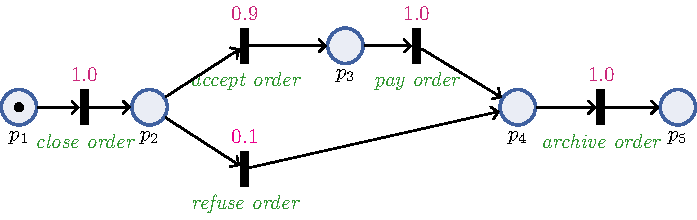
\includegraphics[width=.45\textwidth]{images/petri_tut.pdf}
	\caption{Stochastic Workflow Net modeling our use-case scenario.}\label{fig:petri_tut}
%\vspace{-0.6cm}
\end{figure}
%For example, the probabilistic alignment of a trace with a stochastic net could be represented by the model trace maximizing the combined provision of minimum trace alignment cost and maximum model trace probability. 
With reference to Figure~\ref{fig:petri_tut}, a user might be interested to align the log trace $\langle \textsf{close order},\,\textsf{archive order}\rangle$ with one of the two possible model traces $\langle\textsf{close order},$ $\textsf{accept order},\,\textsf{pay order},\,\textsf{archive order}\rangle$ or $\langle$\textsf{close order}, \textsf{refuse order}, \textsf{archive order}$\rangle$. While the latter trace provides the least alignment cost though the model trace has a low probability ($0.1$), the former gives a slightly greater alignment cost while providing a higher model trace probability ($0.9$). Since, depending on the context, analysts might prefer either the former or the latter alignment, providing a selection of the best $k$ alignments among all the distinct model traces empowers the analysts to find their own trade-off between alignment cost and model trace probability.
%However, in some cases, the user could prefer to identify an alignment with a lower cost even if based on a less probable model trace, while, in other cases, the user could favor a model trace with a higher probability at the expense of a higher alignment cost. Therefore, to provide users with an instrument that allows them to find their own trade-off between alignment cost and model trace probability, we need to return the best $k$ alignments among all the distinct model traces.
%Since when aligning an event log with a stochastic net distinct model traces have different probabilities, the retrieval of the best model trace maximizing the combined provision of minimum trace alignment cost and maximum model trace probability might not suffice. In some cases, indeed, the user could prefer to identify an alignment with a lower cost even if based on a less probable model trace, while, in other cases, the user could favor a model trace with a higher probability at the expense of a higher alignment cost. We consider, therefore, the important tradeoff between both aspects.
%Therefore, in this paper, we propose trace alignment approaches that return the best
To do this, we frame the probabilistic trace alignment problem into the well-known $k$-Nearest Neighbors ($k$NN) problem \cite{Altman} that refers to finding the $k$ nearest data points to a \textit{query} $x$ from a set $\mathcal{X}$ of \textit{data points} via a distance function defined over $\mathcal{X}\cup\{x\}$.
We introduce two ranking strategies. The first one is based on a brute force approach that reuses existing trace aligners  \cite{DBLP:conf/edoc/AdriansyahDA11,LeoniM17} %, where the (optimal) ranking of the top-k alignments is obtained by computing the Levensthein distance between the trace to be aligned and all the model traces and by multiplying each of these distances by the probability of the corresponding model trace. However, even if this approach returns the best trace alignment ranking for a query trace,
requiring to re-compute
 the alignments %must be computed a-new 
 for all the possible traces.% to be aligned. 
 For models generating a large number of model traces, this would clearly become unfeasible: % Therefore, we propose a
 the 
 second strategy %that
  produces an approximate ranking where $x$ and $\mathcal{X}$ are represented as numerical vectors via an embedding $\phi$. 
  %{Then, by exploiting ad-hoc data structures,
%such as Vp-Trees \cite{Fu2000}, Kd-Trees \cite{Maneewongvatana99}, and M-Trees \cite{Ciaccia},
%we can retrieve the neighborhood of $x$ in $\mathcal{X}$ of size $k$  by pre-ordering (\textit{indexing}) $\mathcal{X}$  via a distance between the numerical vectors obtained using $\phi$. 
%Thus, we do not need to analyze the entire space, but just start the search from the top-$1$ alignment. 
If the embeddings $\phi$ for $\mathcal{X}$ are independent of the query of choice $x$, this would not require to constantly recompute the numeric vector representation for $\mathcal{X}$ and to pre-order $\mathcal{X}$ to efficiently visit the search space.
%	
%%%%% Proposed part as the last part of the introduction:
%\texttt{\color{red}[TODO]}
%\todo{this is too specific for an introduction; in particular, too many details on how the experiments are done.}
%We implemented both strategies and perform experiments using a real life event log coming from a hospital system to empirically evaluate the properties of our proposed  strategy. Specifically, we (i) evaluate the correlation between the approximate rankings (using different ways for computing the embeddings) and the optimal ranking, and (ii)~compare the computation time for the exact trace alignment approach against the embedding-based approach. We show that the approximate ranking strategy exploiting a specific data structure (KD-Trees) provides the best trade-off between approximation and execution time, while being more efficient than both the exact ranking and the same approximate ranking with a different data structure (VP-Trees).
%In the next section, we describe the steps required by the tool to compute both alignment strategies. After briefly discussing some preliminary benchmarks, we propose some future work.
\begin{figure}[!t]
	\centering
	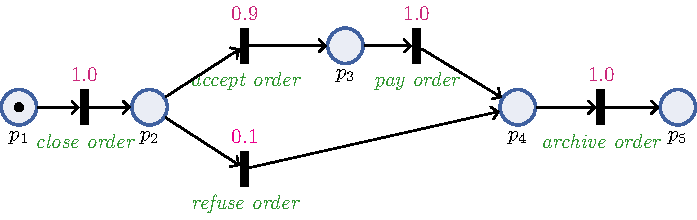
\includegraphics[width=.49\textwidth]{images/petri_tut.pdf}
	\caption{Stochastic Workflow Net modeling our use-case scenario.}\label{fig:petri_tut}
\end{figure}
\begin{figure}[!t]
	\centering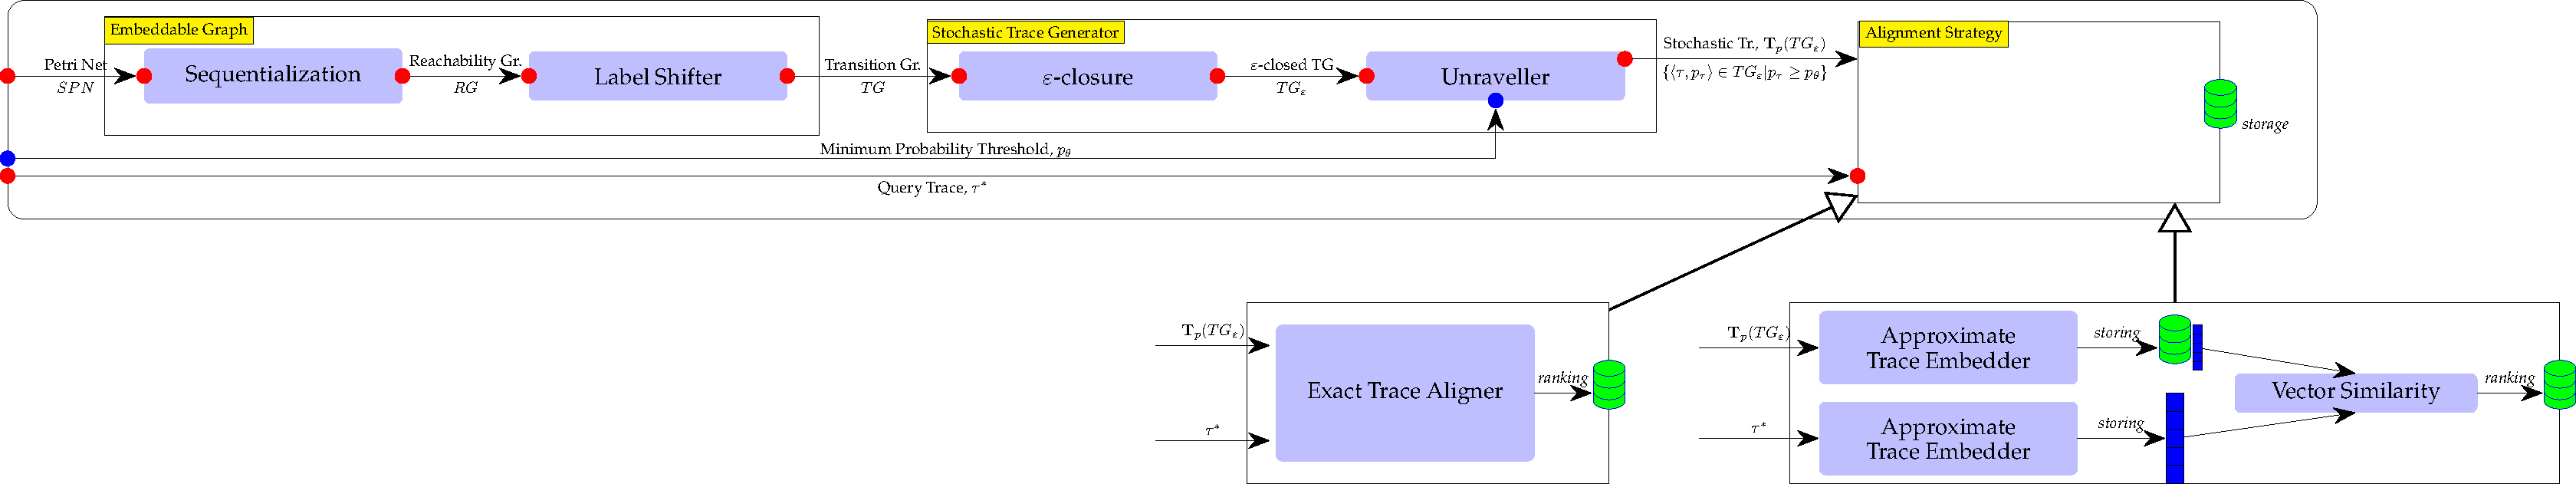
\includegraphics[width=.7\textwidth]{images/pipeline}
	\caption{Proposed pipeline to assess the probabilistic trace alignment.}\label{fig:pipe}
	\vspace*{-0.5cm}
\end{figure}

\section{Probabilistic Trace Alignment Pipeline}
%We now describe the proposed technique for computing probabilistic trace alignments. 
Our approach (\figurename~\ref{fig:pipe}) takes as input
\begin{inparaenum}[\it (i)]
	\item a reference model represented as an Stochastic Workflow Nets $\net$ or an equivalent Transition Graph $G$,
	\item a minimum, positive probability threshold $\pmin \in (0,1]$
	\item a trace $\trace$ of interest,
\end{inparaenum}
and returns a ranking over all the $\net$-traces having a probability greater than or equal to $\pmin$, based on a combined consideration of their probability values and their distance to $\trace$. First, we discuss input formats for \textit{(i)} as in the GUI.


%\section{Modeling Probabilistic Dynamic Systems}
%\label{sec:models}
%In this section, we introduce the different models and techniques that will constitute the basis for representing and computing probabilistic trace alignments.


%\subsection{Input}
%\subsection{Stochastic Workflow Nets}\label{subsec:spn}

\textbf{{Format: \texttt{Petri\_PNML}}.} Petri Nets and Generalized Stochastic Petri Nets are well-established formalisms \cite{DBLP:journals/tosem/PolyvyanyySWCM20} for modelling processes \cite{RoggeSoltiAW13} represented in the Petri Net Markup Language, supported by our tool. Due to the lack of space, we refer to \cite{spdwe} for the usual notation over Petri Nets. We restrict our interest to an interesting class of $1$-\textit{bounded} stochastic Petri nets with no timed transitions, namely \textsc{untimed Stochastic Workflow Nets} denoted as $N$. We now sketch the properties of the SWN accepted in PNML format and loaded as \textsf{PetriNet} objects: we consider two customary markings: the \emph{input} (resp.~\emph{output}) marking $m_{in}$ (resp.~$m_{out}$) assigning a single token to the input (resp.~output) place, and no token elsewhere. We assume to have a set $\alphabet = \tasks \cup \set{\tau}$ of labels, where labels in $\tasks$ indicate process tasks, whereas $\tau$ indicates an invisible execution step ($\tau$-transition). Labels are associated to transitions via a labelling function $\lambda$. A \emph{trace} is a finite sequence of labels from $\tasks$.
%\begin{definition} An \emph{untimed Stochastic Workflow Net (\uswn)}
%	is a tuple $\net = (P,T,F,\ell,W)$ where:
%	\begin{inparaenum}[\itshape (i)]
%		%\begin{inparaenum}
%		\item $(P,T,F)$ is a standard \emph{Workflow net} with places $P$, transitions $T$, and flow relation $F$ such that there is exactly one \emph{input place} with no incoming arc, and exactly one \emph{output place} with no outgoing arcs;
%		\item $\ell: T \rightarrow \alphabet$ is a \emph{labeling function} mapping each transition $t \in T$ into a label $\ell(t) \in \alphabet$ - this either indicates the task executed upon firing $t$, or the fact that $t$ is an invisible transition (in the latter case, $\ell(t) = \tau$);
%		\item $W\colon T\to \mathbb{R}^+$ is a \emph{weight function} assigning a positive firing weight to each transition of the net.
%	\end{inparaenum}
%\end{definition}
%Given an \uswn $\net$, we use dot notation to extract its constitutive components (e.g., $\net.P$ denotes its places). \emph{The same dot notation will be used for the other structures introduced in the paper}. We also use $\net.in$ and $\net.out$ to respectively denote the input and output place of $\net$.
The current state of execution is captured by a marking, i.e., a multiset of places $P$ indicating how many tokens populate each place.
%As pointed out above, \emph{we always assume, as customary in BPM, that the input \uswn is \underline{bounded}}, that is, in every state the number of tokens associated to each place cannot exceed a maximum, fixed threshold.
The notions of transition enablement and firing are also the standard ones  \cite{MarsanCB84}: %, which provides the basis for capturing the stochastic behavior of the net. 
%We use the following notation: given a marking $\marking$ over \uswn $\net$,  $\enaset{\marking}{\net}$ is the set of enabled transitions in $\marking$; given transition $t \in \enaset{\marking}{\net}$, we write $\fire{\marking}{t}{\marking'}{\net}$ to capture the fact that, with, firing $t$ in $\marking$ results in the new marking $\marking'$. A \emph{firing sequence starting from marking $\marking_0$} is a sequence $t_1\cdots t_n$ of transitions from $\net.T$ so that, for every $i \in \set{1,\ldots,n}$, we have that $\fire{\marking_{i-1}}{t_i}{\marking_{i}}{\net}$. We say that the firing sequence results in $\marking_{n}$.
%
given a marking $\marking$ %of $N$ 
and an enabled transition $t \in T_e$, the \emph{firing probability} of $t$ in $\marking$ is $\probt{t}{\marking}{\net} = \frac{W(t)}{\sum_{t'\in T_e}W(t')}$. %As required, 
The probabilities associated to all enabled transitions in a marking always add up to 1.
 A \emph{valid sequence} $\seq = t_1\cdots t_n$ is a firing sequence starting from $m_{in}^\net$ and resulting in $m_{out}$. The probability $\prob{\seq}{\net}$ of a valid sequence is the product of the probabilities associated to each transition: $\prob{\seq}{\net} = \prod_{i \in \set{1,\ldots,n}}\prob{t_i}{\marking_{i-1},\net}$. % A sequence of labels $\run = \alpha_1 \cdots \alpha_n$ from $\alphabet$ is a \emph{run} if there exists a valid underlying sequence $\seq = t_1\cdots t_n$  having $\alpha_i$ as a label for each $t_i\in \seq$. Run $\run$ may have different underlying valid sequences in $\seqs{\run}{\net}$.
  A trace $\trace=\const{a}_1\cdots \const{a}_m$ is a \emph{model trace} (or $\net$-trace for short) if there exists a valid sequence $\seq = t_1\cdots t_n$ where the appended labels $\lambda(t_1)\cdots \lambda(t_n)$ is equivalent to $\trace$ once all the $\tau$-s are stripped.
  %underlying run $\run$ corresponding to $\trace$ once all $\tau$ are removed. 
  There may be multiple valide sequences $\seq\in\seqs{\trace}{\net}$ %$\runs{\trace}{\net}$ 
  underlying an $\net$-trace $\trace$. 
   $\traces{\net}$ is the (possibly infinite) set of $\net$-traces. For a trace $\trace$ of $\net$, its probability $\prob{\trace}{\net}$ is then obtained by collecting all its underlying runs, in turn collecting all their underlying valid sequences, and summing up their respective probabilities: $\prob{\trace}{\net} = %\sum_{\run \in \runs{\trace}{\net}} 
   \sum_{\seq \in \seqs{\trace}{\net}} \prob{\seq}{\net}$. This corresponds to the intuition that, to observe $\trace$, one can equivalently pick any of its underlying valid sequences. Notably, if a trace is not an $\net$-trace (i.e., it does not conform with $\net$), then its probability is 0.
 These structural properties makes them suitable for loading BPMN nets as well: when the \texttt{Petri\_BPMN} is choosen, either the firing weight estimator is constant by default (\texttt{W\_CONSTANT}), or we can choose one from \cite{spdwe}. 
\begin{example} %\small
\label{ex:net}
\figurename~\ref{fig:spn} shows an example of an \uswn with input place $p_1$ and output place $p_7$. One run of the net is $\const{\tau c \tau a a \tau}$, which corresponds to trace $\const{caa}$. Overall, the net supports infinitely many finite traces of the form (represented using regular expressions):
\begin{inparaenum}[\it (i)]
\item $\const{aa^*}$,
\item $\const{cb}$,
\item $\const{caa^*}$.
\end{inparaenum}
\end{example}
%When executing an \uswn, the crucial addition to the standard execution semantics of Workflow nets is that, being the net stochastic, in each marking the set of enabled transitions gets associated to a discrete probability distribution. This is defined as follows: 
%given a marking $\marking$ of $N$ and an enabled transition $t \in \enaset{\marking}{\net}$, the \emph{firing probability} of $t$ in $\marking$ is $\probt{t}{\marking}{\net} = \frac{\net.W(t)}{\sum_{t'\in \enaset{\marking}{\net}}\net.W(t')}$. As required, the probabilities associated to all enabled transitions in a marking always add up to 1.
% %For a run $\run$ of $\net$, its probability $\prob{\seq}{\net}$ is then obtained by summing up the probabilities of all valid sequences corresponding to $\run$: $\prob{\run}{\net} = \sum_{\seq \in \seqs{\run}{\net}} \prob{\seq}{\net}$. Likewise, for a trace $\trace$ of $\net$, its probability is obtained by summing up
% For convenience, when needed, we represent an $\net$-trace as a pair $\tup{\trace,\prob{\trace}{\net}}$, where the probability assigned to $\trace$ by $\net$ is retained.


\textbf{Format: \texttt{StochasticMatrix}.} %\label{subsec:ppn}
The graph and trace embedding techniques %that we will use as the basis for computing probabilistic alignments 
cannot be directly defined over reachability graphs, as they %. In fact, these techniques 
rely on probabilistic \textsc{Transition Graphs} \cite{GartnerFW03} (class \textsf{ReadGraph}). Such graphs have transition probabilities associated to the edges, while nodes have labels in $\Sigma$, 
and represented via transition matrices. Each node is mapped by a matrix $L$ to a single label, as the same label may be used for multiple nodes, while a matrix $R$ represents a probability distribution over the next nodes to be picked upon executing a transition.
%where edges are only labeled by probabilities, whereas labels are attached to nodes. In addition, towards readily enabling efficient algorithmic techniques, such graphs are compactly defined using transition matrixes. We therefore take inspiration from \cite{GartnerFW03} and introduce the so-called \emph{probabilistic transition graphs}, which we will later use to encode \uswn{s} via their reachability graphs.
Due to the lack of space, we refer to \cite{GartnerFW03} for the standard notation for {probabilistic Transition Graphs}:
%For a matrix $Q$ with row set $A$ and column set $B$, notation $[Q]_{ab}$ for $a \in A$ and $b \in B$ denotes the corresponding element in the matrix. In addition $\transp{Q}$ denotes the transposed matrix where rows and columns are inverted. We employ the usual sum and product operations over matrixes and arrays, and denote, for a square matrix $Q$, the repeated multiplication of $Q$ with itself $n$ times by $Q^n$.\todo{Rimuovere questo paragrafo se serve spazio,}\todo{NOn si capisce il significato di $\omega$}
%In our technical treatment, we continue to assume the existence of a set $\alphabet$ of labels (including the special label $\tau$).
%\begin{definition} A \emph{(Probabilistic) Transition Graph} is a tuple $(V,s,t,L,R)$ where:
%	\begin{inparaenum}[\itshape (i)]
%		\item $V \subset \mathbb{N}$ is a set of \emph{nodes};
%		\item $s\in V$ is the \emph{initial node};
%		\item $e\in V$ is the \emph{accepting node};
%		\item $L: \alphabet \times V \rightarrow \{0,1\}$ is a \emph{label matrix} associating each node in $V$ to a single label in $\alphabet$, where for label $\alpha \in \alphabet$ and node $\ind{i} \in V$, $[L]_{\alpha\ind{i}}$ gives $1$ if $\ind{i}$ is labeled by $\alpha$, $0$ otherwise;
%		\item $R: V \times V \rightarrow [0,1]$ is a \emph{(probabilistic) transition matrix} indicating, for each pair of nodes, what is the probability that executing a transition from the first node leads to the second node.
%		% \item $\omega \in [0,1]$ is a \emph{graph weight} indicating an overall value associated to the entire graph.
%	\end{inparaenum}
%	$L$ and $R$ satisfy the following well-formedness conditions:
%	\begin{inparaenum}[\itshape (i)]
%		\item for every $i \in V$ there is one and only one label $\alpha \in \alphabet$ so   that $[L]_{\alpha\ind{i}}=1$;
%		\item  for  every $\ind{i} \in V$, we have that $\sum_{\ind{j}\in V}[R]_{\ind{ij}}=1$.
%	\end{inparaenum}
%\end{definition}
%The condition for $L$ indicates that 
matrices $L$ and $R$ can be exploited to determine the probability of reaching a node labeled by $\beta\in\Sigma$ from any node labeled $\alpha\in\Sigma$ in $n$ steps with $[LR^n\transp{L}]_{\alpha\beta}/[L\transp{L}]_{\alpha\alpha}$, that we can shorthand as $[G.\Lambda^n]_{\alpha\beta}$ \cite{GartnerFW03}.
%
A transition graph $\tg$ can be visualized as shown in \figurename~\ref{fig:lmc}. Still, %The various elements have the obvious interpretation %, with the only important consideration 
%that 
an edge from node $\ind{i}$ to node $\ind{j}$ is only shown if the transition probability $[\tg.R]_{\ind{i}\ind{j}}$ is positive.
%There, each node $\ind{i} \in \tg.V$ is  represented as a circle with its identifying number. The initial node is decorated by a small incoming edge, while the final node is double circled. The label of the node is shown close to the circle, in agreement with $\tg.L$. Finally, an edge from $\ind{i} \in \tg.V$ to $\ind{j} \in \tg.V$ is shown if the transition probability $[\tg.R]_{\ind{i}\ind{j}}$ is positive. Each edge is decorated with the positive probability assigned by $\tg.R$.
%\begin{definition}[Path, trace]
%A \emph{path} in a transition graph $\tg$ is a finite sequence of nodes $\ind{i}_1 \cdots \ind{i}_n$ (with $n > 1$) such that, for every $j \in \set{1,\ldots,n-1}$, we have that $[\tg.R]_{\ind{i}_j\ind{i}_{j+1}} > 0$. Such a path is \emph{valid} if it starts from the initial node and ends in the accepting node of $\tg$, that is, $\ind{i}_1 = \tg.s$ and $\ind{i}_n = \tg.e$.
%
%A \emph{trace} is a finite sequence of nodes that can be turned into a valid sequence by introducing in the sequence an arbitrary number of $\tau$ labels (so as to account for hidden transitions in the graph).
%\end{definition}
%From the definition, it is clear that every valid path can be straightforwardly converted into a corresponding trace by removing all $\tau$ labels from the sequence.
%$\npath{\ind{i}}{\ind{j}}$
%By mirroring to definitions of \uswn{s} taking into account that now labels are on nodes, a \emph{valid sequence} of $\tg$ is a sequence $\ind{i}_0\ldots\ind{i}_n$ of nodes in $\tg.V$ that leads from the initial to the accepting node by only traversing transitions with nonzero probability. 
%\begin{inparaenum}[\it (i)]
%	\item $\ind{i}_0 = \tg.s$;
%	\item $\ind{i}_n = \tg.e$;
%	\item if the sequence contains at least two nodes, each two consecutive nodes are connected by a positive transition probability, i.e., for every $j \in \set{1,\ldots,n}$ we have $[R]_{\ind{i}_{j-1}\ind{i}_{j}} > 0$.
%\end{inparaenum}
Valid sequences and model traces as well as their probability are defined similarly from \uswn{s}, and we employ the same notation. Matrices as well as Linear Algebra operations are implemented using sparse matrices and vectors from Eigen3.

%We close this section by introducing how some  matrix operations defined in the literature \cite{GartnerFW03} are applied to matrixes $L$ and $R$ of $\tg$, towards tackling interesting probability computations. These will be instrumental later on in the paper. Given two nodes $\ind{i},\ind{j} \in \tg.V$, $[R^n]_{\ind{i}\ind{j}}$ returns the probability of having a path in $\tg$ that connects $\ind{i}$ to $\ind{j}$ and has length $n$. Given two labels $\alpha,\beta \in \alphabet$, with $[LR^n\transp{L}]_{\alpha\beta}/[L\transp{L}]_{\alpha\alpha}$, we obtain the probability that, starting in any node labeled by $\alpha$, we reach a node labeled by $\beta$ through  $n$ consecutive steps in $\tg$. As a shortcut notation, we call the result $[\tg.\Lambda^n]_{\alpha\beta}$. Since there may be different nodes labeled by $\alpha$, we need to normalize the resulting probabilities. This is obtained with the division by $L\transp{L}$, which does so by assuming a uniform distribution when picking from which specific $\alpha$-labeled node one wants to start. Notice that these calculations need to be refined so as to consider proper runs and  traces. This will be done in Section~\ref{subsec:as}. %\todo{Rimandare alla sezione giusta}



%
%$\texttt{\color{blue}i}\overset{n}{\rightsquigarrow}\texttt{\color{blue}j}$ of length $n$: therefore, $[\Lambda^n]_{\color{green}\alpha\beta}:=[LR^nL^t]_{\color{green}\alpha\beta}/[LL^t]_{\color{green}\alpha\alpha}$ denotes the probability that, having started at any node labeled $\color{green}\alpha$ and taking $n$ steps, we arrive at any node labeled $\color{green}\beta$ (${\color{green}\alpha}\overset{n}{\rightsquigarrow}{\color{green}\beta}$). We denote as ${\color{green}\alpha}{\rightsquigarrow}{\color{green}\beta}$ an aforementioned path of arbitrary length.
%We can also associate a weight $\omega\in[0,1]\subseteq\mathbb{R}$ to a TG, so to express the probability associated with the TG itself as valid.
%




%\begin{example}
%We can graphically represent such TG as in \cite{Myers1989}.
%Figure \ref{fig:orig} is a  TG $P^*=(\mathtt{\color{blue}1},\mathtt{\color{blue}8},L,R,1)$ where $\omega=1$, where the matrices $L$ and $R$ can be both defined as follows:
%$$L:=\kbordermatrix{
%             & \texttt{\color{blue}1}&\texttt{\color{blue}2}&\texttt{\color{blue}3}&\texttt{\color{blue}4}&\texttt{\color{blue}5}&\texttt{\color{blue}6}&\texttt{\color{blue}7}&\texttt{\color{blue}8}&\texttt{\color{blue}9}&\texttt{\color{blue}10}\\
%\color{green}\varepsilon  & \textbf{1}&0&0&0&0&0&\textbf{1}&\textbf{1}&\textbf{1}&\textbf{1}\\
%\color{green}a            & 0&\textbf{1}&0&\textbf{1}&0&\textbf{1}&0&0&0&0\\
%\color{green}b            & 0&0&0&0&\textbf{1}&0&0&0&0&0\\
%\color{green}c            & 0&0&\textbf{1}&0&0&0&0&0&0&0\\
%}\qquad R:=\kbordermatrix{
%& \texttt{\color{blue}1}&\texttt{\color{blue}2}&\texttt{\color{blue}3}&\texttt{\color{blue}4}&\texttt{\color{blue}5}&\texttt{\color{blue}6}&\texttt{\color{blue}7}&\texttt{\color{blue}8}&\texttt{\color{blue}9}&\texttt{\color{blue}10}\\
%\texttt{\color{blue}1}  & 0&0&{\color{red}p_2}&0&0&0&0&0&{\color{red}p_1}&0\\
%\texttt{\color{blue}2}  & 0&0&0&0&0&{\color{red}p_3}&{\color{red}p_6}&0&0&0\\
%\texttt{\color{blue}3}  & 0&0&0&0&0&0&0&0&0&{\color{red}1}\\
%\texttt{\color{blue}4}  & 0&0&0&0&0&{\color{red}p_3}&{\color{red}p_6}&0&0&0\\
%\texttt{\color{blue}5}  & 0&0&0&0&0&0&0&{\color{red}1}&0&0\\
%\texttt{\color{blue}6}  & 0&0&0&0&0&{\color{red}p_3}&{\color{red}p_6}&0&0&0\\
%\texttt{\color{blue}5}  & 0&0&0&0&0&0&0&{\color{red}1}&0&0\\
%\texttt{\color{blue}8}  & 0&0&0&0&0&0&0&0&0&0\\
%\texttt{\color{blue}9}  & 0&{\color{red}1}&0&0&0&0&0&0&0&0\\
%\texttt{\color{blue}10}  & 0&0&0&{\color{red}p_4}&{\color{red}p_5}&0&0&0&0&0\\
%}$$
%\end{example}

% Given a TG $P=(s,t,L,R,\omega)$, a trace $\tau$ is a tuple in $(\Sigma\backslash\{\varepsilon\})^*$ denoting a path always originating from $s$ and terminating in $t$.
%\subsection{Input Transformation}
\medskip

\textbf{Transforming SWN$\to$TG.} If input is provided as a SWN $N$,  we internally represent all transition firings of an \uswn, together with their probabilities, in a reachability graph $RG(N)$ (\figurename~\ref{fig:rg} and \texttt{PetriMatrix} file format) by interpreting concurrency by interleaving. The transition probability function $P$ assigns to each transition an edge probability in $RG(N)$ as customary.  Due to the lack of space, we skip the customary definition of $RG(N)$.
%\begin{definition}
%The \emph{Reachability Graph} $\rg{\net}$ of \uswn \net is a triple $(M,E,P)$ where:
%\begin{compactitem}[$\bullet$]
%\item $M$ is the set of all reachable markings from $\marking_0^\net$ (including $\marking_0^\net$ itself).
%\item $E \subseteq M \times \alphabet \times M$ is a $\alphabet$-\emph{labeled transition relation} induced by $\net$, that is, for $\marking,\marking' \in M$, we have edge $(\marking,a,\marking') \in E$ if and only if there exists transition $t$  with label $\ell(t) = a$ and such that $\fire{\marking}{t}{\marking'}{\net}$.
%\item $P:E \rightarrow [0,1]$ is the \emph{transition probability} function assigning to each transition $(\marking,a,\marking') \in E$ its corresponding probability, obtained from the firing probability of the \uswn transition(s) that lead from $\marking$ to $\marking'$ and are labeled by $a$: $P(\marking,a,\marking') = \sum_{t_i \in \enaset{\marking}{\net} \text{ s.t.~} \net.\ell(t) = a \text{ and } \fire{\marking}{t}{\marking'}{\net}} \prob{t}{\marking}{\net}$.
%\end{compactitem}
%\end{definition}
%We now need to consider that, 
For a given state, distinct net transitions with the same label might produce the same consequent state, thus becoming indistinguishable from the trace perspective as they collaps into a single edge of the reachability graph. So, we accumulate all their firing probabilities into a single edge value. 
%Next, we handle %need to cope
%%Notice that, in the definition, 
%%we have to account for the possible case where, in a given state, 
%equivalently-labeled distinct net transitions from a given state % with the same label 
%producing the same consequent state: %. In this case, 
%as they are indistinguishable at the trace level by % when observing the execution traces of the net, and in fact they 
%collapsing into a single edge of the reachability graph, %. This is why, in this case, 
%we accumulate all their firing probabilities into a single value.
%
%In the remainder of the paper, 
Given an \uswn $\net$, we always assume that, in addition to its boundedness %, it the following structural assumptions that are natural in the BPM setting:
%\begin{compactitem}
%\item $\net$ is \emph{bounded}, that is, every marking in $\rg{\net}$ assigns at most a pre-defined number of tokens to each place;
%\item 
$\rg{\net}$ does not contain loops where all edges are labeled with $\tau$.
%\end{compactitem}
%The first assumption indicates that a case of the process does not generate unboundedly many parallel threads, and guarantees in turn that the reachability graph contains finitely many states. The second assumption naturally corresponds to how $\tau$-transitions are used when modeling business processes, where they are essential in representing gateways (such as exclusive and parallel splits/joins), cascaded gateways without tasks in between, and skippable tasks.  In all these cases, 
Multiple $\tau$-transitions may be used, but never creating completely invisible loops. {The absence of loops that solely go through $\tau$-transitions is reasonable modeling wise (as skipping multiple times an entire loop iteration is conceptually not distinguishable from not skipping it at all - so we would require there the presence of at least a visible activity witnessing that the iteration was executed, possibly skipping parts of it)}. Under this assumption, % $\net$ enjoys a very interesting property:
 there are only boundedly many valid sequences that can produce a given  trace $\trace$. The probability of $\trace$ can be computed by:
\begin{inparaenum}[\it (i)]
\item exhaustively enumerating all its valid sequences;
\item calculating the probability of each such sequence;
\item summing up all the so-obtained probabilities.
\end{inparaenum}
We directly encode \textsf{PetriNet}s to \textsf{ReadGraph}.
%\figurename~\ref{fig:rg} shows an example of a reachability graph.
\begin{example} %\small
  \label{ex:trace}
Consider the \uswn \net of Example~\ref{ex:net}. Considering trace $\const{caa}$, it is easy to see that it has only one underlying run, namely $\const{\tau c \tau a a \tau}$, in turn produced by a single underlying valid sequence, and that
%The firing probability of picking the first $\tau$-transition starting from the input marking is $1$, as there are no alternatives. In the new marking, where only one token is assigned to $p_2$, the firing probability of choosing the $\tau$-transition above is $\rho_{23} = \frac{v_{\tau_2}}{v_{\tau_2}+v_c}$, whereas that of choosing the $c$-transition below is $\rho_{24} = \frac{v_c}{v_{\tau_2}+v_c}$. Upon choosing the transition below, the new marking assigns only to $p_4$ one token, leaving just one choice to continue by moving that token to $p_6$. In that marking, the probability of choosing the $a$-transition above is $\rho_{65} = \frac{v_{a_3}}{v_{a_3}+v_b}$, resulting in the token being moved to $p_5$. In this new marking, the probability of iterating over the $a$-transition above is $\rho_{55} = \frac{v_{\tau_3}}{v_{\tau_3}+v_{a_2}}$, while that of completing in the output marking via the enabled $\tau$-transition is $\rho_{57} = \frac{v_{\tau_3}}{v_{\tau_3}+v_{a_2}}$. Hence, all in all
$\prob{\const{caa}}{\net} = 1 \cdot \rho_{24} \cdot 1 \cdot \rho_{65} \cdot \rho_{55} \cdot \rho_{57}$.
\end{example}



%Technically:
%\begin{compactitem}
%\item $P$ is a finite set of \textit{places}.
%\item $T$ is a finite set of \textit{transitions}, each of which is associate to a label. Each label either denotes a task executed upon transition firing, or indicates an invisible transition; in the latter case, we employ the special label $\varepsilon$.\footnotesize{This corresponds to the standard notion of $\tau$-transitions in Petri nets, but we use $\varepsilon$ since in the remainder of the paper $\tau$ is used to refer to an execution trace.}
%%to which we associate a label $\lambda(t)\in\Sigma$, where $\Sigma$ also includes the empty string\footnote{Given that we are going to denote the traces as $\tau$ and $t$ as the Petri net Transitions, we choose to denote the empty string as such instead of $\tau$ as in current literature from Petri nets.} $\varepsilon$.
%\item $F\subseteq (P\times T)\cup (T\times P)$ is the flow relation, representing arcs linking places to transitions and transitions to places.
%%to which we associate a \textit{firing cost} $\omega\colon F\to\mathbb{N}$.
%\item The initial place $i\in P$ has no ingoing edges ($\not\exists t\in T. (t,i)\in F$).
%\item The final place $f\in P$ has no outgoing edges ($\not\exists t\in T. (f,t)\in F$).
%\item $W\colon T\to \mathbb{R}^+_{>0}$ defines a \textit{firing weight} associated to each transition.
%\end{compactitem}

%A \textit{marking} is an assignment of a given amount of indistinguishable tokens to places described by a vector $M\colon P\to \mathbb{N}$. We say that a given transition $t$ is \textit{enabled} if $M(p)\geq 1$ for each ingoing $p$ to $t$ ($(p,t)\in F$). If such transition is enabled, then it can \textit{fire} a token. The \textit{enabling transitions} $E(M)$ for a given marking $M$ are all the $t$ reachable from $p$ ($(p,t)\in F$) with $M(p)\neq 0$ where $t$ is enabled. When $t$ can fire a token for a marking $M$, we can generate a novel marking $M'$ from $M$ by moving the tokens from the ingoing places towards the outgoing places as follows:
%\[\forall p\in P.\; M'(p)=M(p)-\mathbf{1}_{(p,t)\in F}+\mathbf{1}_{(t,p)\in F}\]
%We denote the transition from marking $M$ to marking $M'$ via an enabling $t$ as a relation $M\overset{t}{\to}M'$. We say that an \uswn with initial marking $M$ is $k$-\textit{bounded} if each of the markings $M'$ reachable from $M$, $M$ included, have $\forall p\in P.\; M(p)\leq k$\\

\begin{figure*}[!t]
	\begin{minipage}{.49\textwidth}
		\centering
		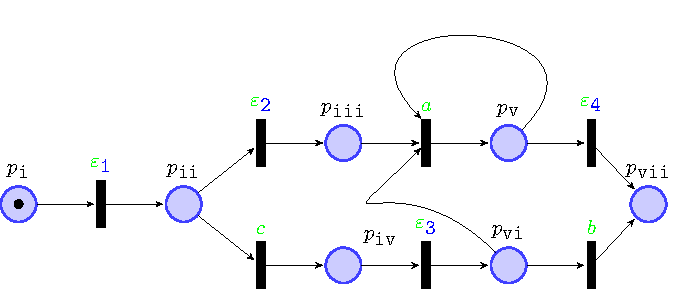
\includegraphics[width=.7\textwidth]{images/petri.pdf}
		\caption{A sample \uswn. Labels are shown in green, $\tau$ transitions in grey, weights in magenta.}\label{fig:spn}
	\end{minipage}\hfill \begin{minipage}{.49\textwidth}\centering
		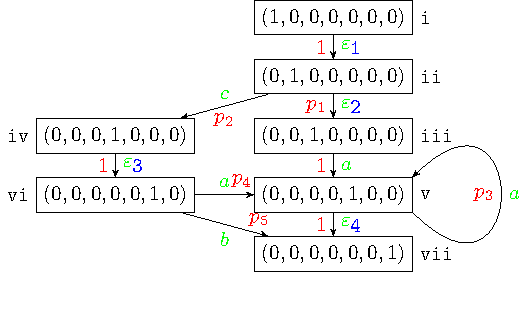
\includegraphics[width=.8\textwidth]{images/rg.pdf}
		\caption{Reachability graph $RG(N)$ of the \uswn $N$. Probabilities are shown in violet.}\label{fig:rg}
	\end{minipage}
\end{figure*} \begin{figure*}[!t]
	\begin{minipage}{.49\textwidth}\centering 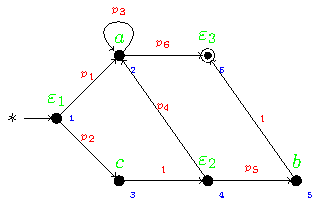
\includegraphics[width=.55\textwidth]{images/running_example.pdf}
	\caption{Transition graph $G_{RG(N)}$ encoding the reachability graph $RG(N)$.}\label{fig:lmc}\label{fig:orig}
\end{minipage}\hfill \begin{minipage}{.49\textwidth}\centering 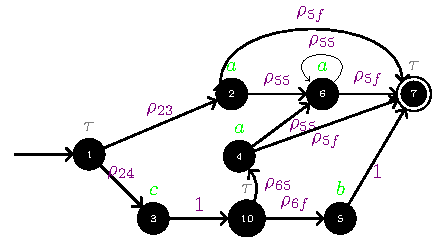
\includegraphics[width=.55\textwidth]{images/closed_example.pdf}
	\caption{Transition graph $\closed{G_{RG(N)}}$ resulting from the transition graph in $G_{RG(N)}$ after $\tau$-closure.}\label{fig:closed}
\end{minipage}
\end{figure*}


%Figures \ref{fig:spn} and \ref{fig:rg} respectively show a sample \uswn and its corresponding reachability graph. This net will be our running example throughout the paper.


%\begin{example}
%Figure \ref{fig:spn} provides a sample \uswn defined as such, and \ref{fig:rg} provides its associated Reachability Graph. This representation can be beneficial when such \uswns are inferred and extracted from log files \cite{PPNFromLog} for extracting the set of the probabilistic traces associated to the \uswn.
%\end{example}
%
%
%We use \uswns for modelling business processes: in fact, it can be shown \cite{RaedtsPUWGS07} that it is always possible to convert BPMNs to \uswns. Last, we also assume that a transition is enabled when all of its input places contain at least one token and that, when a transition fires, we remove one token from each of its input places and depose tokens for each of its output places.

We can show that there exists a conversion from $\rg{\net}$ (\figurename~\ref{fig:rg}) into a transition graph $\tg_{\rg{\net}}$ (\figurename~\ref{fig:orig}) preserving model traces as well as their probabilities via well-known techniques used to \emph{shift labels} from automata theory.  


\textbf{$\tau$-closure} The resulting transition graph $\tg_{\rg{\net}}$ is processed applying a \emph{$\hidden$-closure} that compiles away
$\tau$-transitions. This results into a new transition graph $\closed{\tg_{\rg{\net}}}$ (\figurename~\ref{fig:closed}) %that on the one hand only retains
retaining $\hidden$ labels only in the initial and accepting states while, for the rest, it exclusively operates over visible labels in $\tasks$. %, and, on the other, continues to preserve model traces and their probabilities. Also in this case we omit the details, as 
The transformation relies on well-known automata-based techniques for removing $\epsilon$-moves while preserving model traces, as well as their associated probabilities. %The only non-trivial observation is that, even in our case where probabilities are present, 
All $\tau$ transitions can still be removed thanks to the working hypothesis done for \uswn{s}, as no loops can contain only $\tau$ transitions. %The transition graph in \figurename~\ref{fig:orig} results in that of \figurename~\ref{fig:closed}.
\medskip

\textbf{Unfolding.} Next, we efficiently unfold the previously closed graph to collect TG-traces having probability greater or equal than $\pmin$ (\textsf{Minimum trace probability}) via the Eigen3 linear algebra library. Unfolding is efficiently performed via sparse matrices for TGs over the Eigen library. %The $\hidden$-closed transition graph $\closed{\tg_{\rg{\net}}}$ is \unravelled, so as to collect all the model traces that have a probability of at least $\pmin$. To do so, we rely on a key property that $\closed{\tg_{\rg{\net}}}$ inherits from the fact that it results from an \uswn. 
Since an \uswn has a Workflow net as underlying control-flow structure and given that TG inherits the results from SWNs, no loop can be executed without strictly decreasing the resulting probability. So, all valid sequences with a resulting probability of at least $\pmin$ can be enumerated and returned in a set. The so-obtained sequences are then combined by merging those that produce the same trace, summing up their probabilities, thus obtaining the set of all the traces having a probability greater than or equal to $\pmin$, $\ptraces{\closed{\tg_{\rg{\net}}}}{\pmin}$. The closure operation also implies that the notion of model trace collapses with the one of run modulo removing the initial and the final $\tau$ labels attached to the initial and accepting nodes. %In addition to that, traces might be also pre-filtered by \textsf{Maximum complete trace length}. 
\medskip

%
\subsection{Kernels and Trace Kernels}\label{subsec:katk}
As a foundational basis to compute trace alignments, we adapt similarity measures from the database literature.  Given a set of data examples $\mathcal{X}$, (e.g., strings or traces, transition graphs) a (positive definite) \emph{kernel} function $k\colon \mathcal{X}\times \mathcal{X}\to \mathbb{R}$ denotes the similarity of elements in $\mathcal{X}$. If $\mathcal{X}$ is the $d$-dimensional Euclidean Space $\mathbb{R}^d$, the simplest kernel function is the inner product $\Braket{\mathbf{x},\mathbf{x}'}=\sum_{1\leq i\leq d}\mathbf{x}_i\mathbf{x}'_i$.
A kernel is said to \emph{perform ideally} \cite{Gartner03} when $k(x,x')=1$ whenever $x$ and $x'$ are the same object (\textit{strong equality}) and $k(x,x')=0$ whenever $x$ and $x'$ are distinct objects (\textit{strong dissimilarity}). %A kernel is also said to be \emph{appropriate} when similar elements $x,x'\in\mathcal{X}$ are also close in the feature space. Notice that appropriateness can be only assessed  empirically \cite{Gartner03}.
%A positive definite kernel induces a distance metric as:
%
%When the kernel of choice is the inner product, the resulting distance is the Euclidean distance $\norm{\mathbf{x}-\mathbf{x}'}{2}$. A normalized vector $\hat{\mathbf{x}}$ is defined as $\mathbf{x}/\norm{\mathbf{x}}{2}$. For a normalized vector we can easily prove that: $\norm{\hat{\mathbf{x}}-\hat{\mathbf{x}}'}{2}^2=2(1-\Braket{\hat{\mathbf{x}},\hat{\mathbf{x}}'})$.

When $\mathcal{X}$ does not represent directly a $d$-dimensional Euclidean space, we can use an \emph{embedding} $\embed\colon\mathcal{X}\to \mathbb{R}^d$ to define a kernel $k_\embed\colon \mathcal{X}\times \mathcal{X}\to\mathbb{R}$ as $k_\embed(x,x'):=\Braket{\embed(x),\embed(x')}$. As a result, $k_\embed(x,x')=k_\embed(x',x)$ for each $x,x'\in\mathcal{X}$.

The literature also provides a kernel representation for strings \cite{Gartner03,LodhiSSCW02,GartnerFW03}, which we can directly employ for our traces. We now provide an intuition describing the desired features of this representation \cite{LodhiSSCW02}. If we associate each dimension in $\mathbb{R}^d$ to a different subtrace $\alpha\beta$ of size $2$ (i.e., $2$-grams\footnote{\label{fn:caveat}For our experiments, we choose to consider only $2$-grams, but any $p$-grams of arbitrary length $p\geq 2$ might be adopted \cite{Gartner03}. An increased size of $p$ improves precision but also incurs in a worse computational complexity, as it requires to consider all the arbitrary subtraces of length $p$ whose constitutive elements occur at any distance from each other within the trace.}), the associated coordinate should represent how frequently and ``compactly'' this subtrace is embedded in the trace $\trace$ of interest. Therefore, we introduce a \emph{decay factor} $\lambda\in[0,1]\subseteq\mathbb{R}$ that, for all $m$ subtraces where $\alpha$ and $\beta$ appear in $\trace$ at the same relative distance $L < |\trace|$, weights the resulting embedding as $\lambda^Lm$.

We need to lift this approach so as to consider all occurrences of subtraces $\alpha\beta$ at every distance between $1$ and $|\trace|-1$. To do so, we proceed in two steps. First, we encode $\trace$ into a ``linear'' transition graph $\tg_\trace$ (\figurename~\ref{fig:taustar}) in the obvious way. %\todo{Tagliare dopo i due punti se necessario.} each node in $G_\sigma.V$  corresponds to an element of the trace labeled correspondingly, and the nodes representing two consecutive elements in the trace are connected with a transition probability of 1 (whereas in all the other cases, the probability is 0).
As a second step, we rely on the matrix operations to calculate a simplified version of the embedding defined in \cite{LodhiSSCW02} as $\trembed_{\alpha\beta}(\trace)=\sum_{1\leq i\leq |\trace|}\lambda^i[(\tg_{\trace}.\Lambda)^i]_{\alpha\beta}$. %\todo{No spazio per spiegare cosa succede...}
%This value can be seen as a reward.
The kernel between two traces corresponds to the sum of the products of such values calculated 2-gram by 2-gram for the two traces.
%, namely it is equal to the \emph{kernel convolution}. %\todo{L'ho provato a scrivere intuitivamente, ma non e' chiaro da dove arrivi questo modo di calcolarlo... deriva dalle formule sopra ma la digressione in mezzo e' lunga. Come possiamo fare per chiarire? L'esempio spiega bene tutto!}
This trace kernel returns strong dissimilarity when the two traces have no shared 2-grams at any arbitrary occurring length, but does not enjoy strong equality (as the similarity of a trace with itself is at least $\lambda^2$ - returned when the trace is a 2-gram).

%
%we can represent it as a TG \cite{Myers1989} $(1,{|\tau|},L_\tau,R_\tau,1)$ having $[L_\tau]_{{\color{green}\alpha}\texttt{\color{blue}i}}=1\Leftrightarrow \tau_{\texttt{\color{blue}i}}={\color{green}\alpha}$ and $[L_\tau]_{{\color{green}\alpha}\texttt{\color{blue}i}}=0$ otherwise, and $\forall i<|\tau|.\; [R_\tau]_{\texttt{\color{blue}i(i+1)}}=1 $ and $[R_\tau]_{\texttt{\color{blue}ij}}=0$ otherwise.
%Exploiting this encoding, we can adopt a simplified version of the embedding defined in \cite{LodhiSSCW02,Raedt} as $\embed_{\mathcal{T}}(\tau)_{{\color{green}\alpha\beta}}=\sum_{1\leq i\leq |\tau|}\lambda^i[(\Lambda_\tau)^i]_{\color{green}\alpha\beta}$.
%Please note that this definition is similar to a transition matrix embedding proposed in \cite{GartnerFW03} via geometric series, that is $\sum_i\lambda^i[R^i]_{\color{green}\alpha\beta}$.

\begin{figure}[!t]
	\centering
	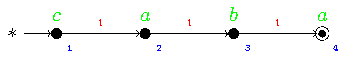
\includegraphics[width=.4\textwidth]{images/taustar.pdf}
	\caption{Graphical representation of the transition graph encoding trace $\const{caba}$.}\label{fig:taustar}

\end{figure}
%
%\begin{example}\label{ex:tracembed}
%	{Let us suppose that we want to align a trace $\tau^*$ to one of the traces from a transition graph: in order to carry out an approximate alignment, we need to transform it to a transition graph first.} A trace $\tau^*=\textup{caba}$ can be graphically represented in Figure \ref{fig:taustar}. The associated TG $T=(\mathtt{\color{blue}1},\mathtt{\color{blue}4},L,R,1)$ has matrices $L$ and $R$  defined as follows:
%	$$L:=\kbordermatrix{
%		& \texttt{\color{blue}1}&\texttt{\color{blue}2}&\texttt{\color{blue}3}&\texttt{\color{blue}4}\\
%		\color{green}a            & 0&\textbf{1}&0&\textbf{1}\\
%		\color{green}b            & 0&0&\textbf{1}&0\\
%		\color{green}c            & \textbf{1}&0&0&0\\
%	}\qquad R:=\kbordermatrix{
%		& \texttt{\color{blue}1}&\texttt{\color{blue}2}&\texttt{\color{blue}3}&\texttt{\color{blue}4}\\
%		\texttt{\color{blue}1}  & 0&\color{red}1&0&0\\
%		\texttt{\color{blue}2}  & 0&0&\color{red}1&0\\
%		\texttt{\color{blue}3}  & 0&0&0&\color{red}1\\
%		\texttt{\color{blue}4}  & 0& 0& 0& 0\\
%	}$$
%We can similarly represent all the traces from the USPN.
%\end{example}

%\begin{example}
%The subtrace \textit{\textbf{\uline{hi}}} is represented in \textit{\textbf{\uline{hi}}deous},   \textit{\uline{\textbf{h}}e\uline{{i}}d\textbf{i}}, and \textit{\uline{{\textbf{h}i}}nd\textbf{i}}, but with different frequencies and subtrace distances. We have $\embed_{\mathcal{T}}(\textit{hideous})_{{\color{green}hi}}=\lambda$,  $\embed_{\mathcal{T}}(\textit{heidi})_{{\color{green}hi}}=\lambda^2+\lambda^4$, and $\embed_{\mathcal{T}}(\textit{hindi})_{{\color{green}hi}}=\lambda+\lambda^4$.
%\end{example}



\begin{table}[t!]
\vspace{+0.7cm}
\caption{Embedding of traces $\const{caba}$, $\const{caa}$ and $\const{cb}$.}\label{tb:embedding}
\vspace{-0.4cm}
\begin{center}
\scalebox{0.6}{
	\begin{tabularx}{\textwidth}{
>{\hsize=.1\hsize}X
>{\hsize=.2\hsize}X
>{\hsize=.1\hsize}X
>{\hsize=.1\hsize}X
>{\hsize=.1\hsize}X
>{\hsize=.1\hsize}X
>{\hsize=.1\hsize}X
>{\hsize=.25\hsize}X
>{\hsize=.2\hsize}X
>{\hsize=.1\hsize}X
}
		\toprule
		& $\const{aa}$    & $\const{ab}$   & $\const{ac}$    & $\const{ba}$   & $\const{bb}$   & $\const{bc}$ & $\const{ca}$ & $\const{cb}$ & $\const{cc}$   \\
		\midrule
		$\const{caba}$ & $\lambda^2$ & $\lambda$ & $0$ & $\lambda$  & $0$  & $0$ & $\lambda+\lambda^3$ & $\lambda^2$ & $0$\\
		%$\const{caaa}$ & $2\lambda+\lambda^2$& $0$ & $0$ & $0$ & $0$ & $0$ & $\lambda+\lambda^2+\lambda^3$ & $0$ & $0$ \\
		$\const{caa}$  & $\lambda$ & $0$ & $0$ & $0$ & $0$ & $0$ & $\lambda+\lambda^2$ & $0$&  $0$\\
		$\const{cb}$   & $0$ & $0$ & $0$ & $0$ & $0$ & $0$ & $0$ & $\lambda$& $0$ \\
		\bottomrule
	\end{tabularx}
}
\vspace{-0.3cm}
\end{center}
\end{table}
\begin{example}\label{ex:wheredotiszero} %\small
Consider tasks $\tasks=\Set{a,b,c}$. The possible 2-grams over $\tasks$ are $\tasks^2=\Set{\const{aa},\const{ab},\const{ac},\const{ba},\const{bb},\const{bc},\const{ca},\const{cb},\const{cc}}$. Table~\ref{tb:embedding} shows the embeddings of some traces. Being a 2-gram, trace $\const{cb}$ has only one nonzero component, namely that corresponding to itself, with $\trembed_{\const{cb}}(\const{cb})=\lambda$. Trace $\const{caa}$ has the 2-gram $\const{ca}$ occurring with length $1$ ($\const{\underline{ca}a}$) and $2$ ($\const{\underline{c}a\underline{a}}$), and the 2-gram $\const{aa}$ with occurring length $1$ ($\const{c\underline{aa}}$). Hence: $\trembed_{\const{ca}}(\const{caa})=\lambda+\lambda^2$ and  $\trembed_{\const{aa}}(\const{caa})=\lambda$.  Similar considerations can be carried out for the other traces in the table.
We now want to compute the similarity between the first trace $\const{caba}$ and the other two traces. To do so, we sum, column by column (that is, 2-gram by 2-gram) the product of the embeddings for each pair of traces. We then get $k_{\trembed}(\const{caba},\const{caa})=\lambda^3+(\lambda+\lambda^3)(\lambda+\lambda^2)$ and $k_{\trembed}(\const{caba},\const{cb})=\lambda^3
$,
%{\footnotesize
%\[
%k_{\trembed}(\const{caba},\const{caaa})=\lambda(\lambda+\lambda^2+\lambda^3)
%~~
%k_{\trembed}(\const{caba},\const{caa})=\lambda(\lambda+\lambda^2)
%~~
%k_{\trembed}(\const{caba},\const{cb})=\lambda(\lambda+\lambda^3)
%\]}
which induces ranking $
k_{\trembed}(\const{caba},\const{caa})>
k_{\trembed}(\const{caba},\const{cb})
$.
\end{example}

\endinput
\subsection{Graph Embedding}\label{ssec:ge}
Graph kernels allow mapping graph data structures to feature spaces (usually an Euclidean space in $\mathbb{R}^n$ for $n\in \mathbb{N}_{>0}$) \cite{Samatova} so to express graph similarity functions that can then be adopted for both classification \cite{TsudaS10} and clustering algorithms. One of the first approaches used in literature involved the definition of topological description vectors \cite{Sidere} for each graph in a graph database, for then defining the graph similarity function as an inner product of their associated vectors. One inconvenience of such a technique is that it is required to perform NP-complete subgraph isomorphisms among a collection of graphs. It has been already proved that the definition of a graph kernel function fully recognizing the structure the graph always boils down to solving such NP-Complete problem \cite{GartnerFW03}, as exact embeddings generable in polynomial can be inferred just for loop-free Direct Acyclic Graphs \cite{BergamiBM20}.


Consequently, most recent literature focused on extracting relevant features of such graphs, that are then used to define a graph similarity function. The most common approach adopted in the kernel to extract such features is called \textit{propositionalization}: we might extract all the possible features (e.g., subsequences), and then define a kernel function based on the occurrence and similarity of these features \cite{Gartner03}.
% !TeX root=../main.tex
\begin{figure}[!t]
	\hspace*{-1cm}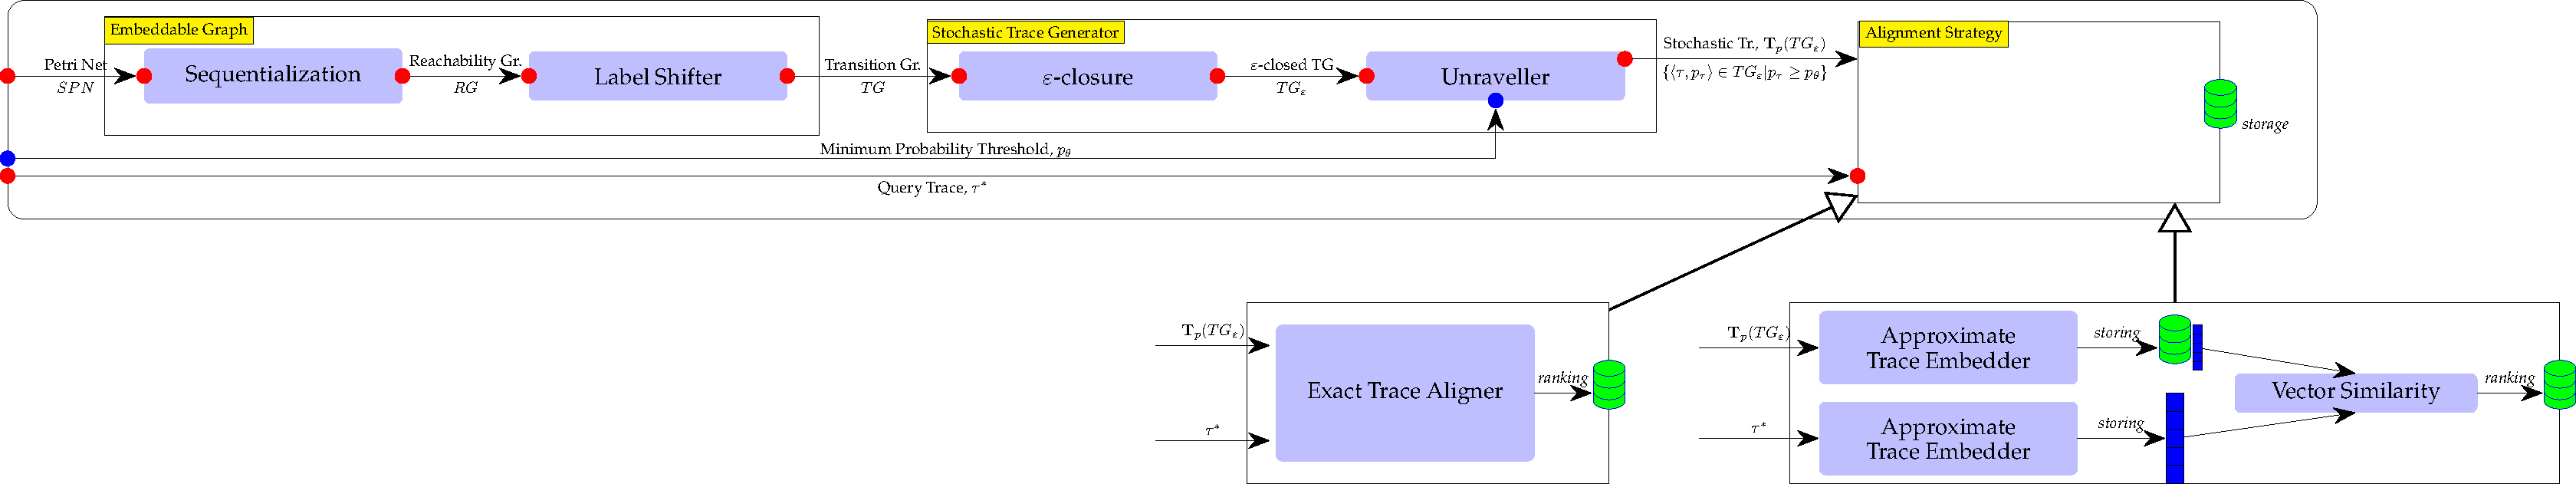
\includegraphics[width=1.2\textwidth]{images/pipeline}
	\caption{Proposed pipeline to assess the Probabilistic Trace Alignment}\label{fig:pipe}
\end{figure}


\section{Probabilistic Trace Alignment Pipeline}
We propose the pipeline from Figure \ref{fig:pipe} connecting several existing formalizations via intermediate processing steps.
The input of this pipeline is a query trace to be aligned, an \uswn, and a minimum probability threshold $\pmin$. Its output
is a set of model traces satisfying $\pmin$ with an alignment ranking.
%
The pipeline has the following phases: after representing the \uswn as a graph of all the sequentially scheduled transitions
(\S\ref{sec:seqZ}), we shift the labels from the edges towards the nodes while preserving the set of probabilistic traces
(\S\ref{sec:LSift}) and minimize the graph representation by removing the $\tau$-labelled nodes while preserving the
trace probability (\S\ref{sec:clos}). We extract the set of all traces having probability above $\pmin$ threshold (\S\ref{sec:unrav}) and  apply two different alignment strategies; one exact  (\S\ref{subsec:eta}), and one approximated.


We later discuss how to rank traces in the exact and approximated scenarios by reducing the alignment process to a k-nearest
neighbor problem. While the exact trace alignment requires to perform the alignment process each time a novel trace $\sigma^*$ is
introduced (\S\ref{subsec:exbkptap}), the approximated alignment can split the alignment into a preliminary loading phase and a
query phase. In the former, each stochastic trace from the \uswn is represented as a vector (\S\ref{subsec:ate}), and in the latter the to-be-aligned trace $\sigma^*$ is first represented as a vector and then compared to all the other vectorial representations.

\subsection{Sequentialization}\label{sec:seqZ}
The sequentialization step transforms an \uswn with an initial marking $M$ into a Reachability Graph $(\mathcal{M},\mathcal{E})$
generated by a sequentialization process, where potentially concurrent firing transitions are represented via a sequential scheduling.

\begin{definition}[Reachability Graph]
	Given an initial marking $M$ for an \uswn $\mathcal{U}$,  the \textit{Reachability Graph} for $\mathcal{U}$ is a graph
	$(\mathcal{M},\mathcal{E})$ where the nodes  $\mathcal{M}$ are composed of all the reachable markings from $M$,
	and the edges $\mathcal{E}$ are induced by the aforementioned relation $M\overset{t}{\to}M'$ among the
	nodes. To each edge $M\overset{t}{\to}M'$, we associate a transition probability $\mathbb{P}\left(M\overset{t}{\to}M'\right)=\frac{W(t)}{\sum_{t'\in E(M)}W(t')}$ \cite{spdwe}.
\end{definition}

\begin{example}
From the \uswn in Figure \ref{fig:spn}, the sequentialization process generates the reachability graph depicted in
Figure \ref{fig:rg}. Each node represents a marking $M$ as a vector, and the edges are labelled with the firing transitions.
The edges associated to this graph describe potentially concurrent firing transitions sequentially. While visiting the graph from
$M$, the chaining of the edge labels generates a trace produced from the untimed Workflow Net, and the product of the edge
weights provides the probability associated to the trace.
\end{example}



\subsection{Label Shifter}\label{sec:LSift}
Reachability graphs obtained via sequentialization cannot be directly embedded using existing methods:  Reachability graphs
associated to stochastic workflow nets are edge labelled, but TGs are node labelled. To represent the former as the latter, we
shift the labels from the edges to the nodes  while preserving the set of traces and their associated probability.
Such transformation is defined next.

\begin{definition}[Label Shifter]\label{def:transf}
The reachability graph $(\mathcal{M},\mathcal{E})$ generated from an initial marking $M$, is transformed into the TG $(s,t,L,R,1)$, where:
\begin{itemize}
	\item If is a single edge $M_1\overset{t}{\to}M_2\in\mathcal{E}$ where $M_1=M$, then $s=M\overset{t}{\to}M_2$; otherwise, define a new node $\textbf{i}$ and set it as the initial node for TG: $s=\textbf{i}$.
	\item If is a single edge $M_1\overset{t}{\to}M_2\in\mathcal{E}$ without outgoing edges in the reachability graph, then $t=M_1\overset{t}{\to}M_2$; otherwise, define a new node $\textbf{f}$ and set it as the accepting node for TG:  $t=\textbf{f}$.
	\item $[L]_{\lambda(t),\;M\overset{t}{\to} M'}=1$ for each $M\overset{t}{\to} M'\in\mathcal{E}$; if $\textbf{i}$ is defined then $[L]_{\tau\textbf{i}}=1$; if $\textbf{f}$ is defined, then $[L]_{\tau\textbf{f}}=1$; $[L]_{ij}=0$ otherwise.
	\item $[R]_{M\overset{t}{\to} M',\;M'\overset{t'}{\to} M''}=\frac{W(t')}{\sum_{\textbf{t}\in E(M')}W(\textbf{t})}$ for each $M\overset{t}{\to} M',M'\overset{t'}{\to} M''\in\mathcal{E}$; if $\textbf{i}$ is defined, $[R]_{\textbf{i},\;M\overset{t}{\to}M'}=\frac{W(t)}{\sum_{\textbf{t}\in E(M)}W(\textbf{t})}$; if $\textbf{f}$ is defined, then $[R]_{M\overset{t}{\to}M',\;\textbf{i}}=1$ for each $M'$ without outgoing edges in the reachability graph; $[R]_{ij}=0$ ow.
\end{itemize}
\end{definition}

\endinput
%
We can show that the TG obtained in Definition \ref{def:transf} preserves the same set of probabilistic traces associated by the reachability graph. The proof is omitted due to the lack of space.

\begin{example}
Figure \ref{fig:lmc} shows the TG obtained from the reachability graph in Figure \ref{fig:rg}. Nodes are labelled with the firing
transition labels (in green), and edges preserve the probabilistic information from the reachability graph (in red). Intuitively, when a
new initial node \textit{\textbf{i}} is inserted, we preserve all the initial probabilistic choices that a transition is fired from an initial
marking $M$, while the intermediate edges inherit the probabilisitc choice of the firing transition from the subsequent choices. When
a new final node \textit{\textbf{f}} is added, such edges always have probability $1$, and thus do not interfere with the
initial traces' probability.
\end{example}

\subsection{$\tau$-closure}\label{sec:clos}
The $\tau$-closure process has two main purposes: first, reduce the size of the previously generated TG by removing all
$\tau$-labelled nodes \texttt{\color{blue}w} and preserving the connection between  the nodes \texttt{\color{blue}u}
from its ingoing edges   $\texttt{\color{blue}u}\xrightarrow{\color{violet}\rho}\texttt{\color{blue}w}$ with the nodes \texttt{\color{blue}v} from its ingoing edges   $\texttt{\color{blue}w}\xrightarrow{\color{violet}\rho'}\texttt{\color{blue}v}$ by establishing new edges $\texttt{\color{blue}u}\xrightarrow{\color{violet}\rho\rho'}\texttt{\color{blue}v}$. $\tau$-labelled initial (or accepting) nodes are removed iff they have only one outgoing (ingoing) edge with probability $1$.

\begin{example}\todo{Is it now ok?}
	The $\tau$-closure removes the non-initial and non-accepting nodes within an automaton, while preserving the probabilistic trace equivalence of the two automata. Let us suppose to apply the $\tau$-closure to the automata in Figure \ref{fig:orig}: node \texttt{\color{blue}10} is removed alongside its associated edges, and new edges $\texttt{\color{blue}3}\xrightarrow{\color{violet}\rho_{65}}\texttt{\color{blue}4}$ and $\texttt{\color{blue}3}\xrightarrow{\color{violet}\rho_{6f}}\texttt{\color{blue}5}$ are introduced. The resulting TG $P$ is represented with the same graphical depiction Figure \ref{fig:closed}.
\end{example}
%
Consequently, it is always possible to minimize a TG  via $\tau$-closure, so that the only nodes labelled as $\tau$
are the source and the target nodes and the set of weighted traces is preserved. From now on, we consider only minimised TGs.

\subsection{Unraveller}\label{sec:unrav}
%Being that both the graph isomorphism problem is NP-Complete and the
Since TGs are fully characterized by the set of the probabilistic traces that they generate,  we say that two TGs are
(probabilistic-trace) equivalent iff they share the same set of weighted traces. In particular, we denote as $\mathcal{W}_p^n(P)$ the set of all the weighted traces in $P$ having at least probability $p$ and maximum length $n$. Under these assumptions, the probabilistic trace equivalence is deterministic.

\begin{example}
	The set $\mathcal{W}_0^{\aleph_0}(P^*)$ of weighted traces of the TG in Figure \ref{fig:orig} is
%	The TG in Figure \ref{fig:orig} has the following set $\mathcal{W}_0^{\aleph_0}(P^*)$ of weighted traces:
$$\set{\braket{\underbrace{\color{green}a\dots a}_{n},{\color{violet}\pa\pc^n\pf}}|n\in \mathbb{N}_{>0}}\cup \set{\braket{{\color{green}c}\underbrace{\color{green}a\dots a}_{n},{\color{violet}\pb\pd\pc^n\pf}}|n\in \mathbb{N}_{>0}}\cup\{\braket{{\color{green}cb},{\color{violet}\pb\pe}}\}$$
After the $\tau$-closure process, $\mathcal{W}_0^{\aleph_0}(P^*)=\mathcal{W}_0^{\aleph_0}(P)$, so the two TGs are (probabilistic-trace) equivalent.
\end{example}

% !TeX root=../main.tex
%\vspace{-0.5cm}
%As mentioned in the introduction, 
%When aligning a log trace with an \uswn, the retrieval of the best model trace maximizing the combined provision of minimum trace alignment cost and maximum model trace probability might not suffice. 
%An alignment of a trace with an \uswn could be represented by the best model trace maximizing the combined provision of minimum trace alignment cost and maximum model trace probability. However, in some cases, the user could prefer to identify an alignment with a lower cost even if based on a less probable model trace, while, in other cases, the user could favor a model trace with a higher probability at the expense of a higher alignment cost.
%Therefore, we need to return the best $k$ alignments among all the distinct \unravelled\ model traces in $\ptraces{\net}{\pmin}=\ptraces{\closed{\tg_{\rg{\net}}}}{\pmin}$. 
In the database community, this problem is usually tackled via $k$-Nearest Neighbors ($k$NN) that refers to finding the $k$ nearest data points to a \textit{query} $x$ from a set $\mathcal{X}$ of \textit{data points} via a distance function $d_k$ defined over $\mathcal{X}\cup\{x\}$. {In particular, by exploiting ad-hoc data structures, such as VP-Trees and KD-Trees, %VP-Trees \cite{Fu2000} \cite{Maneewongvatana99}, and M-Trees \cite{Ciaccia},
we can retrieve the neighborhood of $x$ in $\mathcal{X}$ of size $k$ by pre-ordering (\textit{indexing}) $\mathcal{X}$ via $d_k$ and starting the search from the top-$1$ alignment.

%Usually, $x$ and $\mathcal{X}$ are represented as numerical vectors via an embedding $\phi$. {By exploiting ad-hoc data structures such as Vp-Trees \cite{Fu2000}, Kd-Trees \cite{Maneewongvatana99}, and M-Trees \cite{Ciaccia}, we can retrieve the neighborhood of $x$ in $\mathcal{X}$ of size $k$  by pre-ordering (\textit{indexing}) $\mathcal{X}$  via $d_k$. Thus, we do not need to analyze the entire space, but just start the search from the top-$1$ alignment. We prefer embeddings $\phi$ for $\mathcal{X}$ that are independent of the query of choice $x$, as it would not require to constantly change the numeric vector representation for $\mathcal{X}$.

%The well-known $k$-nearest neighbors ($k$NN) problem \cite{Altman} refers to finding the $k$ nearest data points to a \textit{query} $x$ from a set $\mathcal{X}$ of \textit{data points} via a distance function $d_k$ defined over $\mathcal{X}\cup\{x\}$. Usually, $x$ and $\mathcal{X}$ are represented as numerical vectors via an embedding $\phi$. {By exploiting ad-hoc data structures such as Vp-Trees \cite{Fu2000}, Kd-Trees \cite{Maneewongvatana99}, and M-Trees \cite{Ciaccia}, we can retrieve the neighborhood of $x$ in $\mathcal{X}$ of size $k$  by pre-ordering (\textit{indexing}) $\mathcal{X}$  via $d_k$. Thus, we do not need to analyze the entire space, but just start the search from the top-$1$ alignment. We prefer embeddings $\phi$ for $\mathcal{X}$ that are independent of the query of choice $x$, as it would not require to constantly change the numeric vector representation for $\mathcal{X}$.
%	
%If we want to align a trace $\logtrace$ over the \unravelled\ traces $\mathcal{X}=\WCal{\pmin}{n}$,
%the $k$-Nearest Neighbors describe the best $k$ alignments for $\logtrace$.} We discuss two strategies for obtaining the
%top-$k$ trace alignments.


%\begin{figure*}[!t]
%	\begin{minipage}{.49\textwidth}
%		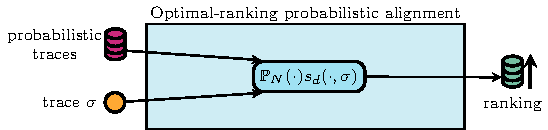
\includegraphics[width=\textwidth]{images/aligner_exact.pdf}
%		\caption{Optimal-Ranking Trace Aligner.}\label{fig:optimal}
%	\end{minipage}\hfill \begin{minipage}{.49\textwidth}
		
%		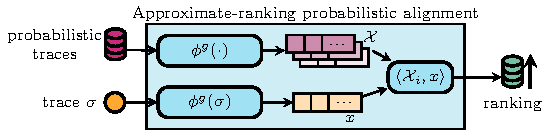
\includegraphics[width=\textwidth]{images/aligner.pdf}
%		\caption{Approx.-Ranking Trace Aligner.}\label{fig:approximate}
%	\end{minipage}
%\end{figure*}
%\vspace{-0.6cm}

\noindent
\textbf{1) Optimal-Ranking Trace Aligner.}\label{subsec:eta}
%One way to probabilistically align traces is to 
By reusing existing trace aligners  \cite{DBLP:conf/edoc/AdriansyahDA11,LeoniM17} providing an alignment cost  $d(\logtrace,\nonlogtrace)$ between model and log traces as the Levenshtein distance and
%, i.e., the {minimum} cost for aligning one of the two traces with respect to the other when all the possible moves have cost equal to 1.\footnote{This is slightly different from the Levenshtein distance from the literature since here the replacement is obtained as a concatenation of a deletion and an addition.}
using the decision theory, a we can express the ranking as a preliminary ranked distance $\probskip{\nonlogtrace} d(\logtrace,\nonlogtrace)$, considering both the alignment cost and the model trace probability.
%
We can represent it 
%To represent the same intuition of such a weighted distance 
as a ranking function %, we must transform it into a
%similarity function 
returning $1$ when $\nonlogtrace=\logtrace$ and $\probskip{\logtrace}=1$ hold. We then express $d$ as
%\xout{We can express our probabilistic trace alignment as finding the trace that maximizes both the trace's probability and its similarity with the query trace $\logtrace$. Still, the trace alignments problems are usually expressed via trace alignments cost functions, and not via trace similarities \cite{LeoniM17}. Given a generic trace cost function $d(\trace,\trace')$, it is always possible to convert it into}
a normalized similarity score $s_d(\logtrace,\nonlogtrace):=\frac{1}{d(\logtrace,\nonlogtrace)+1}$. %The maximum similarity is reached when the distance is $0$ and the similarity decreases while the distance increases. %\xout{As a consequence, the exact trace aligner will find the weighted trace $\braket{\trace,\mathbb{P}(\trace)}$ in $\mathcal{W}_{\pmin}(P)$ maximising $s_d(\trace,\logtrace)$, and use $s_d$ as a ranking function.} \ADD
{The golden ranking function (i.e., the one producing the optimal ranking) can therefore be represented as $\goldenrank(\logtrace,\nonlogtrace)=\probskip{\nonlogtrace} \probskip{\logtrace} s_d(\logtrace,\nonlogtrace)$. Such function can be exploited to generate the best optimal-ranking trace alignment for a log trace $\logtrace$, where $\goldenrank$ must be computed a-new for all the possible $\logtrace$.
	
	
\noindent
\textbf{2) Approximate-Ranking Trace Embedder.}\label{subsec:ate}
%Ranking optimality comes at the sub-optimal cost of a brute-force recomputation of $\goldenrank$ for each novel trace $\logtrace$ to align.
%\footnote{By embedding  all the \unravelled\ model traces via $\phi_{\logtrace}(\nonlogtrace)=\Big(\frac{1}{\probskip{\nonlogtrace}\sqrt{\probskip{\nonlogtrace}^2+s_d^2(\logtrace,\nonlogtrace)}},\frac{1}{s_d(\logtrace,\nonlogtrace)\sqrt{\probskip{\nonlogtrace}^2+s_d^2(\logtrace,\nonlogtrace)}}\Big)$ over a specific $\logtrace$, by representing  $\logtrace$ as $(0,0)$, and by using the Euclidean Distance as a distance, we ensure that all the neighbors of $(0,0)$ will represent the top-$k$ best alignments for $\logtrace$.}. %This is not optimal for $k$NN-based techniques, as this entails the  redefinition of the multidimensional search space $\mathcal{X}$ for each new alignment $\logtrace$. The ``recomputation cost'' could be completely avoided by providing an embedding strategy $\gorgembed$ that is independent of the to-be-aligned trace $\logtrace$.
Since each embedding $\phi$ entails an associated similarity metric $k_\phi$, %and hence an associated
%distance $d_{k_\phi}$ (Equation \ref{eq:dofk}), 
we can compute the embeddings for all the \unravelled\ traces
before performing the top-$k$ search ensuring that they are independent of the trace to align, thus avoiding the brute-force cost. This computational gain comes with a loss in precision %, as the generation of precise embeddings for graph data with loops is an NP-Complete (thus intractable) problem
 \cite{GartnerFW03} and, in its approximated version, is not able to accurately represent the data using low-dimensional vectors \cite{Seshadhri5631}. %So, our proposed embedding (that we indicate with $\gorgembed$) is weakly-ideal.
Differently from some graph embedding literature, we are interested in neither embedding one single node of the graph, nor in providing a vector representation of the whole graph. While these are common strategies for graph embeddings, we want to represent TG traces,  which might be composed by different valid sequences (paths), as vectors.  We are also interested in the intersection of embedding strategies for whole node-labeled graphs with string embedding traces, as we use vectors to compare TG traces with log traces. 
{To obtain our proposed embedding $\gorgembed$, we hence adapt the  embedding strategy} $\trembed$ from \cite{LodhiSSCW02} {by addressing some short\-comings: %that this strategy presents:}
%\begin{alphalist}
% \item it does not perform weakly-ideally, so we cannot numerically assess if two embeddings represent equivalent traces;
% \item it does not characterize $\tau$-moves, so the probabilities of the initial and final $\tau$-moves are not preserved;
% \item it is affected by numerical errors from finite arithmetics: longer traces $\nonlogtrace$ generated from skewed probability distributions $\expN.\Lambda^i$ suffer from greater truncation errors, as smaller $\lambda^i$ components for bigger $i<|\nonlogtrace|$ will be ignored, preventing a complete numerical vector characterization of  $\nonlogtrace$ in practice.
%\end{alphalist}
%
%{To overcome these shortcomings we} 
we
\begin{alphalist} \item propose a weakly-ideal embedding \cite{Gartner03} which, differently from current literature, \item exploits an
$\omega$ factor for preserving probabilities from and to $\tau$ transitions. We also \item mitigate the
numerical truncation errors induced by trace length and probability distribution skewness through two sub-embedding strategies,
$\epsilon^x$ and $\nu^x$, where the former descends from $\trembed$ and the latter approximates the trace similarity via label frequencies similarity.
\end{alphalist}
Since a model trace embedding  adequately representing the transitions in our implementation requires an intermediate $G$ representation, we map each $\nonlogtrace$ to a pair $(\tg_\nonlogtrace,\omega)$}, where \begin{inparaenum}[\it (i)]
\item $\tg_\nonlogtrace$ is a transition graph containing all the paths describing $\nonlogtrace$, where all $\tau$-labelled nodes are removed, while
\item the graph weight $\omega$ preserves the weight of the possible initial and final edges that were removed due to the former requirement.
\end{inparaenum}

%The formal definition of such operation is omitted due to the lack of space.
%Please observe that the first requirement is mandatory, as present string embedding strategy do not cope with silent characters $\tau$.
%
%
%
%
%	\begin{definition}[$\closed{G}$ projection over traces]
%		Given a minimum probability thre\-shold $\pmin$ and a $\tau$-closed transition graph $\closed{G}=(V,s,t,L,R)$, for each trace $\nonlogtrace\in\ptraces{\closed{G}}{\pmin}$, the $\closed{G}$ projection over $\nonlogtrace$ is a pair ($\closed{G}_\nonlogtrace,\omega)$, where $\closed{G}_\nonlogtrace$ is a transition graph such that
%\begin{inparaenum}[\it (i)]
%	\item $\closed{G}_\nonlogtrace.V$ contains all distinct nodes generating $\nonlogtrace$ from $\closed{G}$	(i.e., $\bigcup_{\xi\in\runs{\nonlogtrace}{\closed{G}}}\seqs{\xi}{ \closed{G}}$);
%	\item $\closed{G}_\nonlogtrace.s = s$;
%	\item  $\closed{G}_\nonlogtrace.t = t$;
%	\item $\closed{G}_\nonlogtrace.L$ (and $\closed{G}_\nonlogtrace.R$) is the submatrix of $L$ (and $R$) over the columns (and rows) in $\closed{G}_\nonlogtrace.V$, and $\omega \in [0,1]$ is a \emph{graph weight} preserving the transition probabilities from and to $\tau$ nodes and computed as $1-\prod_{\xi\in\runs{\sigma}{\closed{G}},\eta\in\seqs{\xi}{\closed{G}}}\Big(1-(\textit{ifte}([L]_{\tau\eta_1},[R]_{\eta_1\eta_2})$
%	 $\textit{ifte}([L]_{\tau t_n},[R]_{t_{n-1} t_n})\Big)$,
%	where $\textit{ifte}(x,y):=x(y-1)+1$ returns $y$ if $x=1$ and $1$ otherwise. We denote the set of all the $\closed{G}_\nonlogtrace$ as $\TBf{\pmin}{4}(\closed{G})$.
%\end{inparaenum}
%\dots
%		
%		\dots we generate a set $\TBf{\pmin}{n}(\closed{G})$ of projected TGs $P$ for each trace in $\WCal{\pmin}{n}(P)$ as follows: for each weighted trace $\braket{\nonlogtrace,\probskip{\nonlogtrace}}\in\WCal{\pmin}{n}(P)$ generated from a path $\pi_\nonlogtrace=s\to n_2\rightsquigarrow n_m\to t$ over $R$, we generate a TG $P_\nonlogtrace=(s',t',L_\nonlogtrace,R_\nonlogtrace,\omega')$, where \begin{inparaenum}[\it (i)]
%			\item $s'=s$ if $\textit{label}(s)\neq \tau$ and $t'=n_2$ otherwise,
%			\item $t'=t$ if $\textit{label}(t)\neq \tau$ and $t'=n_m$ otherwise,
%			\item $L_\nonlogtrace$ (and $R_\nonlogtrace$) is the submatrix of $L$ (and $R$) over the non-$\tau$ labeled notes in $\pi_\nonlogtrace$ and the labels from $\nonlogtrace$,
%			\item $\omega'$ is initialized by $\omega$ and then multiplied by $[R]_{s,n_2}$ (and also $[R]_{n_m,t}$) if $\textit{label}(s)=\tau$ (and  $\textit{label}(t)=\tau$).
%		\end{inparaenum}
%\end{definition}
%	
\begin{table}[!t]
	\setlength{\textfloatsep}{-1pt}
	\caption{Projections of $\expN$ over $\net$-traces of length $4$.}\label{tab:proj}
	\centering
	\resizebox{.3\textwidth}{!}{\begin{tabular}{>{\centering\arraybackslash} m{1cm}| >{\centering\arraybackslash} m{4cm} >{\centering\arraybackslash} m{1cm} >{\centering\arraybackslash} m{1cm} }
			\toprule
			$\nonlogtrace$&$G_\nonlogtrace$&$l$&$\omega$\\
			\midrule
			$\const{a}$ & 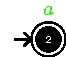
\includegraphics{images/trace_a} & $1$ & $\color{violet}\pa\pf$\\
			$\const{cb}$ & 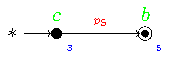
\includegraphics{images/trace_cb} & $2$ & $\color{violet}\pb$\\
			$\const{aaa}$ & 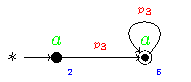
\includegraphics{images/trace_a_loop} & $3$ & $\color{violet}\pa\pf$\\
			$\const{caa}$ & 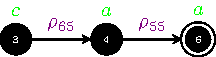
\includegraphics{images/trace_caa} & $3$ & $\color{violet}\pb\pf$\\
			\bottomrule
	\end{tabular}}\qquad \qquad 	
	\resizebox{.3\textwidth}{!}{\begin{tabular}{>{\centering\arraybackslash} m{1cm}| >{\centering\arraybackslash} m{4cm} >{\centering\arraybackslash} m{1cm} >{\centering\arraybackslash} m{1cm} }
	\toprule
	$\nonlogtrace$&$G_\nonlogtrace$&$l$&$\omega$\\
	\midrule
	$\const{aa}$ & 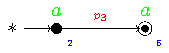
\includegraphics{images/trace_aa} & $2$ & $\color{violet}\pa\pf$\\
	$\const{ca}$ & 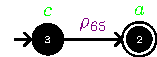
\includegraphics{images/trace_ca} & $2$ & $\color{violet}\pb\pf$\\
	\begin{tabular}{l}aaaa\end{tabular} & 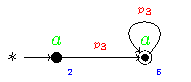
\includegraphics{images/trace_a_loop} & $4$ & $\color{violet}\pa\pf$\\
	$\const{caaa}$ & 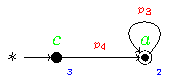
\includegraphics{images/trace_ca_loop} & $4$ & $\color{violet}\pb\pf$\\
	\bottomrule
\end{tabular}}
\end{table}
%The graph weight $\omega$ derives from the outgoing edges of the initial node and the ingoing edges of the accepting node when such nodes are labeled as $\tau$. Given that (i) the embedding strategy from \cite{LodhiSSCW02} allows trace embedding only for visible (i.e., non-$\tau$) transitions, and (ii) the trace extraction process discards the $\tau$ information, we use $\omega$ to preserve such information.
%We call the pair consisting of a transition graph and a graph weight a \emph{weighted transition graph}.
\begin{example}\label{ex:neue}
Given the $\tau$-closed transition graph $\closed{\tg_{\rg{\net}}}$ resulting from the process model, we assign the probability values
$\pa=0.8$, $\pb=0.2$, $\pc=\pf=0.5$, $\pd=0.7$, and $\pe=0.3$. The $\ptraces{\expN}{0}$ with maximum length $4$ are:
%$$\begin{aligned}
%\ptraces{\expN}{0}_{|\nonlogtrace|\leq 4}=
$\{\braket{\const{a},0.4},\braket{\const{aa},0.2}$, $\braket{\const{aaa},0.1}$, $\braket{\const{ca},0.07}$, $\braket{\const{cb},0.06}$,
$\braket{\const{aaaa},0.05},\braket{\const{caa},0.035},\braket{\const{caaa},0.0175}\}$.
%\end{aligned}$$
Table \ref{tab:proj} shows the projected transition graphs associated to such traces, where only the relevant information
for embedding them is displayed (e.g., all the $\tau$-labeled nodes are removed).
\end{example}
	
{Our proposed embedding $\gorgembed$ is computed for each pair $(\tg_\nonlogtrace,\omega)$ generated from each unfolded trace %transition graph generated in the former definition. The goal is to use
%$k_{\gorgembed}$ for ranking all the traces generated by \unravelling\ via such graphs. 
We can now extend the embedding $\trembed$ \cite{LodhiSSCW02} by including the traces associated probability, and making the ranking induced by $k_{\gorgembed}$ the inverse of the ranking induced by the
sum of the following distances: the transition correlations $\epsilon$ and the transition label frequency $\nu$.}
%\xout{Given that we previously observed that a TGs $\closed{\tg_{\rg{\net}}}$ can be fully characterized (read, similarity) by their associated set of traces $\mathcal{W}_p^n(P)$  and that the trace embedding can be described as an embedding over a TG, we can characterize a TG embedding as a transition matrix embedding. In addition to that, when two Workflow Nets share similar node labelings but no ${\color{green}\alpha}\rightsquigarrow{\color{green}\beta}$ paths for any ${\color{green}\alpha}$ and ${\color{green}\beta}$, we should combine the former embedding with an embedding characterizing the frequency on how the nodes' labels appear in the generated traces.} \ADD
{We also require that the desired properties of $\gorgembed$ are independent of the characterization of $\epsilon$ over the $2$-grams in $\mathcal{A}^2$ and $\nu$ over the labels in $\mathcal{A}$, which  provide different embedding strategies. } Therefore, our proposed $\gorgembed$ embedding is defined as follows:


%\begin{table}[!t]
%	\centering
%	\caption{Embedding representation for the TG $P$ in \figurename~\ref{fig:closed} and the trace $\logtrace=\textup{caba}$ after representing it as in \figurename~\ref{fig:sigmastar}. Please note that we restrict $\trace_\tau^2$ to the one from $P$.}\label{tab:emb1}
%		\begin{tabular}{l|l|l|l|l|l|l|}
%	\toprule
%	& a    & b                                                   & c    & aa   & ca   & cb   \\
%	\midrule
%	$\gorgembed(P)$ & $9.94\cdot10^{-25}$ & $1.18\cdot 10^{-26}$ & $1.04\cdot10^{-25}$ & $4.45\cdot 10^{-25}$ & $6.22\cdot10^{-25}$ & $8.29\cdot10^{-26}$\\
%	$\gorgembed(P_{\logtrace})$ & $8.16\cdot10^{-17}$ & $4.08\cdot 10^{-17}$ & $4.08\cdot10^{-17}$ & $4.37\cdot 10^{-17}$ & $1.03\cdot10^{-16}$ & $4.37\cdot10^{-17}$\\
%	\bottomrule
%\end{tabular}
%\end{table}
\begin{definition}[G-Embedding]\label{def:ppne}
%Given a finite set of non-empty labels $\trace_\tau =\trace\backslash\{\tau\}$, $\trace_\tau^2$ denotes all the possible pair of labels associated to paths ${\color{green}\alpha}\rightsquigarrow{\color{green}\beta}$ and $\trace_\tau$ denotes the set of all the possible non-$\tau$ node labels. Therefore, it is always possible to enumerate $\trace_\tau^2\cup\trace_\tau$ via an enumeration by a bijection $\iota\colon \trace_\tau^2\cup\trace_\tau\to  N$, where $N\subset \mathbb{N}_{\neq 0}$ and $\max N=|N|$.
Given a $\closed{G}$ projection over $\nonlogtrace$ ($\closed{G}_\nonlogtrace,\omega)$ and a tuning parameter $t_f\in[0,1]\subseteq\mathbb{R}^+_{0}$, the \emph{G-Embedding} $\gorgembed$ %over the visible $2$-grams and transition labels, $\mathcal{A}\cup\mathcal{A}^2$, 
exploiting the matrix represantion of\cite{GartnerFW03} in $\nu$ and $\epsilon$ for TGs is defined as
$$\gorgembed_{i}(\closed{G}_\nonlogtrace)=\begin{cases}
	\omega \frac{\epsilon_\const{ab}(\closed{G}_\nonlogtrace)}{\|\epsilon\|_2}\;t_f^{|R>0|}\, & {i}=\const{ab}\\
	\frac{\nu_\const{a}(\closed{G}_\nonlogtrace)}{\|\nu\|_2}\;\;\;\,t_f^{|R>0|}\, & {i}=\const{a}\\
\end{cases}$$
\end{definition}
%
Here, the kernel function associated to such embedding can be exploited to return the best approximated trace alignment for a log trace represented as $G_{\logtrace}$. %\xout{Similarly, we can provide the TG $P\in\mathbf{P}$ providing the best approximated alignment for $P_{\logtrace}$ as $\underset{P}{\max\arg}\underset{ P_\trace\in\mathbf{P}_p^n(P)}{\max} k_{\gorgembed}(P_\trace, P_{\logtrace})$.}¯
%
\begin{table}[!t]
	\caption{Different sub-embedding definitions ($\epsilon^1$, $\epsilon^2$, $\nu^1$, and $\nu^2$) for $\gorgembed$.}\label{tab:embedstrat}
	\centering
	\resizebox{.6\textwidth}{!}{\begin{tabular}{c|c|c}
		\toprule
		& $x=1$ & $x=2$ \\
		\midrule
		$\epsilon^x_\const{ab}(\overline{G}_\nonlogtrace):=$ & $\label{eq:epsilon}
		\sum_{i=1}^l{\lambda^i}\frac{[LR^iL^t]_\const{ab}}{\sum_{\const{a'b'}\in\mathcal{A}^2}R^i_\const{a'b'}}$ & $
		\sum_{i=1}^l\lambda^i[\Lambda^i]_\const{ab}$\\
		$\nu^x_\const{a}(\overline{G}_\nonlogtrace):=$ & $\frac{1}{c}\sum_{\nonlogtrace'\in \ptraces{\closed{G}_\nonlogtrace}{0}}\frac{|\Set{\nonlogtrace_i'\in\nonlogtrace'|\const{a}\in\mathcal{A}\wedge \nonlogtrace'_i=\const{a}}|}{|\nonlogtrace'|}$ & $0$ \\
		\bottomrule
	\end{tabular}}
\end{table}
%
For sub-embeddings $\epsilon$ and $\nu$  we choose two possible interchangeable definitions ($x=1$ and $x=2$) shown in Table \ref{tab:embedstrat}: here, $l$ is the path length (reported in Table \ref{tab:proj}), and $c$ for $\nu^1$ is a normalization factor such that $\sum_{\const{a}\in\mathcal{A}}\nu^1_\const{a}(P)=1$. While $\nu^2$ implies to completely ignore the label frequency contribution, $\epsilon^2$ is the direct implementation of $\trembed$ from \cite{LodhiSSCW02}, and $\epsilon^1$ and $\epsilon^2$ only differ from the normalization perspective. %In Example \ref{ex:cmpexample}, we will see that the given definition of $\epsilon^1$ provides a better approximation than the edge embedding $\epsilon^2$.
%
$t_f\in [0,1]\subseteq\mathbb{R}^+_{0}$ (\textsf{Tuning}) and $\lambda\in [0,1]\subset\mathbb{R}^+_{0}$ (\textsf{Lambda}) are tuning parameters that can be
inferred from the available data \cite{DriessensRG06}. The latter describes the previously mentioned decay factor, while $t_f$
represents the relevance of our embedding representation as the number of edges within $\closed{G}_\nonlogtrace$ increases. In our experiments and
examples, we choose $t_f=0.0001$ and $\lambda=0.07$. Omitted proofs show that our embedding  performs weakly-ideally. 
%This representation is independent of the representation associated with a trace to be aligned. Therefore it does not have to be recomputed at each alignment with a different $\logtrace$.



%When the transition matrix is ergodic \cite{StocasticCC},  the transition matrix embedding converges to $\epsilon(R)_{\color{green}\alpha\beta}=[(\mathbf{I}-\lambda\Lambda)^{-1}]_{\color{green}\alpha\beta}$ \cite{GartnerFW03} for $n\to+\infty$.
%\begin{table}[!t]
%	\centering
%\vspace{+0.2cm}
%	\caption{Embeddings for $\net$-traces of maximum length $4$ and $\logtrace=\const{caba}$.}\label{tab:emb2}\label{tab:embsitar}
%	\resizebox{\textwidth}{!}{\begin{tabular}{lllllllllllll}
%		\toprule
%		& $\const{a}$    & $\const{b}$                                                   & $\const{c}$    & $\const{aa}$  & $\const{ab}$   & $\const{ac}$   & $\const{ba}$  & $\const{bb}$   & $\const{bc}$   & $\const{ca}$   & $\const{cb}$  & $\const{cc}$  \\
%		\midrule		
%		$\gorgembed(\overline{G}_\const{aaaa})$ & $1.00\cdot 10^{-24}$ & $0.00\cdot 10^{0}$   & $0.00\cdot 10^{0}$   & $6.44\cdot 10^{-26}$ & $0.00\cdot 10^{0}$& $0.00\cdot 10^{0}$& $0.00\cdot 10^{0}$& $0.00\cdot 10^{0}$& $0.00\cdot 10^{0}$    &$0.00\cdot 10^{0}$& $0.00\cdot 10^{0}$& $0.00\cdot 10^{0}$ \\
%		$\gorgembed(\overline{G}_\const{aaa})$  & $1.00\cdot 10^{-24}$ & $0.00\cdot 10^{0}$   & $0.00\cdot 10^{0}$   & $1.29\cdot 10^{-25}$ & $0.00\cdot 10^{0}$& $0.00\cdot 10^{0}$& $0.00\cdot 10^{0}$& $0.00\cdot 10^{0}$& $0.00\cdot 10^{0}$    &$0.00\cdot 10^{0}$& $0.00\cdot 10^{0}$& $0.00\cdot 10^{0}$ \\
%		$\gorgembed(\overline{G}_\const{aa})$   & $1.00\cdot 10^{-24}$ & $0.00\cdot 10^{0}$   & $0.00\cdot 10^{0}$   & $2.57\cdot 10^{-25}$ & $0.00\cdot 10^{0}$& $0.00\cdot 10^{0}$& $0.00\cdot 10^{0}$& $0.00\cdot 10^{0}$& $0.00\cdot 10^{0}$    &$0.00\cdot 10^{0}$& $0.00\cdot 10^{0}$& $0.00\cdot 10^{0}$ \\
%		$\gorgembed(\overline{G}_\const{a})$    & $1.00\cdot 10^{-4}$  & $0.00\cdot 10^{0}$   & $0.00\cdot 10^{0}$   & $0.00\cdot 10^{0}$   & $0.00\cdot 10^{0}$& $0.00\cdot 10^{0}$& $0.00\cdot 10^{0}$& $0.00\cdot 10^{0}$& $0.00\cdot 10^{0}$    &$0.00\cdot 10^{0}$& $0.00\cdot 10^{0}$& $0.00\cdot 10^{0}$ \\
%		$\gorgembed(\overline{G}_\const{caa})$  & $7.07\cdot 10^{-25}$ & $0.00\cdot 10^{0}$   & $7.07\cdot 10^{-25}$ & $1.46\cdot 10^{-25}$ & $0.00\cdot 10^{0}$& $0.00\cdot 10^{0}$& $0.00\cdot 10^{0}$& $0.00\cdot 10^{0}$& $0.00\cdot 10^{0}$    &$2.05\cdot 10^{-25}$& $0.00\cdot 10^{0}$& $0.00\cdot 10^{0}$ \\
%		$\gorgembed(\overline{G}_\const{ca})$   & $7.07\cdot 10^{-25}$ & $0.00\cdot 10^{0}$   & $7.07\cdot 10^{-25}$ & $0.00\cdot 10^{0}$   & $0.00\cdot 10^{0}$& $0.00\cdot 10^{0}$& $0.00\cdot 10^{0}$& $0.00\cdot 10^{0}$& $0.00\cdot 10^{0}$    &$1.00\cdot 10^{-8}$& $0.00\cdot 10^{0}$& $0.00\cdot 10^{0}$ \\
%		$\gorgembed(\overline{G}_\const{cb})$   & $0.00\cdot 10^{0}$   & $7.07\cdot 10^{-25}$ & $7.07\cdot 10^{-25}$ & $0.00\cdot 10^{0}$   & $0.00\cdot 10^{0}$& $0.00\cdot 10^{0}$& $0.00\cdot 10^{0}$& $0.00\cdot 10^{0}$& $0.00\cdot 10^{0}$    &$0.00\cdot 10^{0}$ & $4.29\cdot 10^{-9}$& $0.00\cdot 10^{0}$ \\
%		$\gorgembed(\overline{G}_\const{caaa})$ & $7.07\cdot 10^{-25}$ & $0.00\cdot 10^{0}$   & $7.07\cdot 10^{-25}$ & $1.03\cdot 10^{-25}$ & $0.00\cdot 10^{0}$& $0.00\cdot 10^{0}$& $0.00\cdot 10^{0}$& $0.00\cdot 10^{0}$& $0.00\cdot 10^{0}$    &$7.20\cdot 10^{-26}$ & $0.00\cdot 10^{0}$& $0.00\cdot 10^{0}$ \\
%		\bottomrule
%				$\gorgembed(\overline{G}_\const{caba})$ & $8.16\cdot10^{-17}$ & $4.08\cdot 10^{-17}$ & $4.08\cdot10^{-17}$ & $4.37\cdot 10^{-17}$ &  $0.00\cdot 10^{0}$& $0.00\cdot 10^{0}$& $0.00\cdot 10^{0}$ & $0.00\cdot 10^{0}$ & $0.00\cdot 10^{0}$    & $1.03\cdot10^{-16}$ & $4.37\cdot10^{-17}$& $0.00\cdot 10^{0}$ \\
%		\bottomrule
%	\end{tabular}}
%
%\end{table}%
%\xout{After defining the embedding, we can show that this embedding establishes some desired features that are independent of the definition of $\epsilon$ and $\nu$, and that $\epsilon$ and $\nu$ only depend on the characterization of both the labelling $L$ and the transition matrix $R$. We provide a rewriting proposition that is going to be used in the incoming subsection to provide the aforementioned characterizing properties.} \ADD
%
%Given that kernel functions $k_\phi$ are defined as the dot product between the embedding $\phi$ of distinct objects $x$ (\S\ref{subsec:katk}), then we can express the kernel $k_{\gorgembed}$ as such dot product and, after normalizing $\epsilon$ and $\nu$, we can rewrite such kernel
%
%%
%\begin{proposition}\label{lem:rewritinglemma}
%Given $(\overline{G}_\sigma,\omega)$ and $(\overline{G}_{\nonlogtrace},\omega')$ with $\overline{G}_\sigma=(s,t,L,R)$ and $\overline{G}_{\nonlogtrace}=(s',t',L',R')$, the definition for $k_\gorgembed$ is expanded as follows:
%$$
%k_{\gorgembed}(\overline{G}_\sigma,\overline{G}_{\nonlogtrace})=\omega\omega't_f^{|R>0|+|R'>0|}\left(1-\frac{\norm{\hat{\epsilon}-\hat{\epsilon}'}{2}^2}{2}\right)+t_f^{|R>0|+|R'>0|}\left(1-\frac{\norm{\hat{\nu}-\hat{\nu}'}{2}^2}{2}\right)\\$$
%\end{proposition}
%\begin{proof} We can close the goal by definition of $k_{\phi}$ as a vector dot product for any embedding $\phi$ and by  $\|\hat{\mathbf{x}}-\hat{\mathbf{x}}'\|_2^2=(2-1\braket{\hat{\mathbf{x}},\hat{\mathbf{x}}'})$ (\S\ref{subsec:katk}).	
%%	
%%	 for normalized vectors (\S\ref{subsec:katk}), we can expand the former definition as follows:
%%$$\begin{aligned}
%%{k_{\gorgembed}(P,P')}&{=\Braket{\gorgembed(P),\gorgembed(P')}}\\
%%	&{=\sum_{\alpha\beta\in \trace_\tau^2}\frac{\epsilon_{\color{green}\alpha\beta}}{\|\epsilon\|_2}\frac{{\epsilon'}_{\color{green}\alpha\beta}}{\|\epsilon'\|_2}\omega\omega't_f^{|R>0|+|R'>0|}\quad+\quad \sum_{\alpha\in \trace_\tau}\frac{\nu_{\color{green}\alpha}}{\|\nu\|_2}\frac{{\nu'}_{\color{green}\alpha}}{\|\nu'\|_2}t_f^{|R>0|+|R'>0|}}\\
%%	&{=ww'\trace^{|Rb>0|+|R'>0|}\sum_{\alpha\beta\in \trace_\tau^2}\frac{\epsilon_{\color{green}\alpha\beta}}{\|\epsilon\|_2}\frac{{\epsilon'}_{\color{green}\alpha\beta}}{\|\epsilon'\|_2}\quad+\quad t_f^{|R>0|+|R'>0|}\sum_{\alpha\in \trace_\tau}\frac{\nu_{\color{green}\alpha}}{\|\nu\|_2}\frac{{\nu'}_{\color{green}\alpha}}{\|\nu'\|_2}}\\
%%	&{=\omega\omega't_f^{|R>0|+|R'>0|}\Braket{\hat{\epsilon}, \hat{\epsilon}'}+ t_f^{|R>0|+|R'>0|}\Braket{\hat{\nu}, \hat{\nu}'}}\\
%%	&{=\omega\omega't_f^{|R>0|+|R'>0|}\left(1-\frac{\norm{\hat{\epsilon}- \hat{\epsilon}'}{2}^2}{2}\right)+ t_f^{|R>0|+|R'>0|}\left(1-\frac{\norm{\hat{\nu}- \hat{\nu}'}{2}^2}{2}\right)}\\
%%\end{aligned}$$
%\end{proof}
%%

%\xout{Given that we can now follow Definition \ref{def:ppne} for representing a trace $\trace$ as a proper embedding after transforming it as a TG $P_{\logtrace}$ (\S\ref{subsec:katk}), we can find the TG $P$ providing the best approximate match with  a trace $\trace$ as follows:}
%\[\Rcancel{\underset{{P}}{\max\arg}\;k_{\gorgembed}(P,T)}\]
%\xout{Still, this TG matching strategy does not allow to find the trace maximizing such score.} %To assess such problem, the next section is going to determine both an exact (\S\ref{subsec:exbkptap}) and an approximated strategy (\S\ref{subsec:akptap}) for probabilistically matching one single trace from the TG.
%
%\xout{Given the characterization of a TG as in \S\ref{subsec:ppn} and the embedding strategy proposed in Definition \ref{def:ppne}, We can \ADD{now} generate an embedding for each possible weighted trace $\braket{\trace,\probskip{\trace}}\in\mathcal{W}_p^n(P)$ for a given TG $P$ as described in the following definition:}





\begin{table}[!t]
\vspace{+1.3mm}
	\caption{Comparison between the ranking induced by the optimal ranking $\goldenrank$ and the proposed kernel $k_{\gorgembed}$ with embedding strategies $\epsilon^1$ and $\nu^1$: arrows $\boldsymbol{\downarrow}$ remark the column of choice under which we sort the rows.}\label{tab:rank3}
	\centering
	%	\begin{tabular}{l|c|ll}
	%		\toprule
	%		$\trace$ & $k_{\gorgembed}(\trace,\logtrace)$ & \textit{kernel ranking} & expected ranking\\
	%		\midrule
	%		a & $8.16\cdot 10^{-21}$ & \textbf{1} & \textbf{\color{blue}1}\\
	%		ca & $1.89\cdot 10^{-24}$ & \textbf{2} & \textbf{\color{blue}4}\\
	%		cb & $7.64\cdot 10^{-25}$ & \textbf{3} & \textbf{\color{blue}5}\\
	%		caa & $1.14\cdot 10^{-40}$ & \textbf{4} & \textbf{\color{blue}7}\\
	%		caaa & $9.84\cdot 10^{-41}$ & \textbf{5} & \textbf{\color{blue}8}\\
	%		aa & $9.28\cdot 10^{-41}$ & \textbf{6} & \textbf{\color{red}2}\\
	%		aaa & $8.72\cdot 10^{-41}$ & \textbf{7} & \textbf{\color{red}3}\\
	%		aaaa & $8.44\cdot 10^{-41}$ & \textbf{8} & \textbf{\color{red}6}\\
	%		
	%		\bottomrule
	%	\end{tabular}
	
	\resizebox{.6\textwidth}{!}{\begin{tabular}{l|ll|cc}
		\toprule
		
		{$\nonlogtrace$} &
		%\multirow{2}{*}{$d(\trace,\logtrace)$} &
		%\multicolumn{2}{c|}{$\mu_{\logtrace}$} &
		$( \probskip{\nonlogtrace}$ &  $,\,\boldsymbol{\downarrow} s_d(\logtrace,\nonlogtrace)) $ &
		{$=\goldenrank(\logtrace,\nonlogtrace)$} &
		{$k_{\gorgembed}(\closed{G}_\logtrace,\closed{G}_{\nonlogtrace})$} \\
		
		
		\midrule
		$\const{caa}$  & $0.035$ & $\;\; 0.8333$ & $0.0292$ & $1.14\cdot 10^{-40}$\\
		$\const{caaa}$  &  $0.0175$ & $\;\; 0.8333$ & $0.0145$ & $9.84\cdot 10^{-41}$\\
		$\const{a}$  & $0.4$ & $\;\; 0.6250$  & $0.2500$ & $8.16\cdot 10^{-21}$ \\
		$\const{aaaa}$  & $0.05$ & $\;\; 0.6250$ & $0.0357$ & $8.44\cdot 10^{-41}$\\
		$\const{aa}$  & $0.2$ & $\;\; 0.7142$ & $0.1428$ & $9.28\cdot 10^{-41}$ \\
		$\const{aaa}$  & $0.1$ & $\;\; 0.7142$ & $0.0714$ & $8.72\cdot 10^{-41}$\\
		$\const{ca}$  &  $0.07$ & $\;\; 0.7142$ & $0.0500$ & $1.89\cdot 10^{-24}$\\
		$\const{cb}$  &  $0.06$ & $\;\; 0.7142$ & $0.0428$ & $7.64\cdot 10^{-25}$\\
		\bottomrule
	\end{tabular}\quad \begin{tabular}{l|c}
	\toprule
	
	{$\nonlogtrace$} &
	{$\boldsymbol{\downarrow}\goldenrank(\logtrace,\nonlogtrace)$} \\
	
	
	\midrule
	$\const{\color{blue}a}$  &  $0.2500$ \\
	$\const{\color{red}aa}$  &  $0.1428$  \\
	$\const{\color{red}aaa}$  & $0.0714$ \\
	$\const{\color{blue}ca}$  &   $0.0500$\\
	$\const{\color{blue}cb}$  & $0.0428$ \\
	$\const{\color{red}aaaa}$  &  $0.0357$ \\
	$\const{\color{blue}caa}$  &  $0.0292$ \\
	$\const{\color{blue}caaa}$  &   $0.0145$ \\
	\bottomrule
\end{tabular}\quad	\begin{tabular}{l|c}
	\toprule
	
	{$\nonlogtrace$} &
	{$\boldsymbol{\downarrow}k_{\gorgembed}(\closed{G}_\logtrace,\closed{G}_{\nonlogtrace})$} \\

	
	\midrule
	$\const{\color{blue}a}$  & $8.16\cdot 10^{-21}$ \\
	$\const{\color{blue}ca}$  &   $1.89\cdot 10^{-24}$\\
	$\const{\color{blue}cb}$  &   $7.64\cdot 10^{-25}$\\
	$\const{\color{blue}caa}$  &$1.14\cdot 10^{-40}$\\
	$\const{\color{blue}caaa}$  &  $9.84\cdot 10^{-41}$\\
	$\const{\color{red}aa}$  &  $9.28\cdot 10^{-41}$ \\
	$\const{\color{red}aaaa}$  & $8.44\cdot 10^{-41}$\\
	$\const{\color{red}aaa}$  &  $8.72\cdot 10^{-41}$\\
	\bottomrule
\end{tabular}}
\end{table}




\begin{example}%\small \label{ex:11}
	\vspace{0.2cm}
%Table \ref{tab:emb2} shows the embeddings $\gorgembed(\overline{G}_\nonlogtrace)$ generated from Example \ref{ex:neue}, where the $l=|\nonlogtrace|$ for each $\unravelled$ trace $\nonlogtrace$.
%{After representing trace $\logtrace=\const{caba}$ to be aligned as a graph (\figurename~\ref{fig:taustar}), we can represent its}
%%\xout{Similar considerations can be also drawn from the}
%embedding $\gorgembed(\overline{G}_{\logtrace})$ with strategies $\epsilon^1$ and $\nu^1$ %\xout{associated to the trace $\logtrace=\textup{caba}$ (also in Table --):} \ADD
%{as} in Table \ref{tab:embsitar}: $\const{a}$ is clearly the most frequent label while $\const{b}$ and $\const{c}$ are equiprobable. The $2$-gram $\const{ca}$ appears twice in the trace set and then, it is more frequent than the remaining $2$-grams.
	The dot product $k_{\gorgembed}(\logtrace,\nonlogtrace)=\braket{\gorgembed(\overline{G}_\logtrace),\;\gorgembed(\overline{G}_{\nonlogtrace})}$ with sub-embed\-ding $\nu^1$ and $\epsilon^1$, for each trace $\nonlogtrace\in\WCal{0}{4}_{|\sigma'|\leq 4}$, are represented in Table \ref{tab:rank3}. %, where an explicit computation of $\gorgembed(\overline{G}_\logtrace)$ is omitted due to lack of space to the benefit of optimal ranking $\goldenrank$. 
	$k_{\gorgembed}$ approximates the optimal ranking as it tends to rank the transition graphs $\closed{G}_\nonlogtrace$ (generated from $\overline{G}$ via projection) similarly to the $\net$-traces over $\mathcal{R}$. In the same table, the ranking similarities shared between the two different ranking strategies are highlighted in blue, while the most evident ranking discrepancies are marked in red. Such similarities and differences can be assessed via Spearman Correlation Index \cite{BergamiBM20}. Evaluations exploiting such index were removed due to lack of space; our future work will include those as well as temporal benchmarks.
\vspace{0cm}
\end{example}


%\begin{example}\label{ex:moreskew}
%	\xout{Let us suppose to change the probability distribution associated with the $P$'s edges, so that it becomes more skewed and that some traces are relatively more probable than others. Let us set $p_1=p_2=0.5$, $p_3=0.9$, $p_6=0.1$, $p_4=0.3$, and $p_5=0.7$, so that the initial choice is equiprobable but performing a loop is more probable than terminating the path. We keep the other tuning parameters as in Example \ref{ex:withpaths}. In this case, we generate the following set of weighted traces:}
%	$$\begin{aligned}
%	\Rcancel{\mathcal{W}_0^4(P)=\{}&\Rcancel{\braket{cb,0.35},\braket{a,0.05},\braket{aa,0.045},\braket{aaa,0.0405},}\\
%	&\Rcancel{\braket{aaaa,0.03645},\braket{ca,0.015},\braket{caa,0.0135},\braket{caaa,0.01215}\}}\\
%	\end{aligned}$$
%	\xout{Let us also assume that we want to align these traces in a probabilistic way with the query $\logtrace=\textup{caba}$: the distance ($d$) and similarity ($s_d$) scores will be still the same, while the associated probabilities will vary. The expected ranking by multiplying weight with similarity is represented in Table \ref{tab:witherror}.}
%	
%	%\xout{As a consequence of the different probability distribution associated to the edges, a different set of embedding will be generated for each trace of interest while the TG $T$ associated to $\logtrace$ will be kept the same. Table \ref{tab:witherror} represents the ranking induced by the kernel $k_{\gorgembed}$ over this different set of vectors by ranking the traces in descendant order of $k_{\gorgembed}$. As we might notice, the more skewed edge probability distribution introduced more errors in the ranking result: while the largest ranking subsequence (marked in blue) always starts from the best-expected trace \textit{cb}, this element now appears in the third position, and the position of traces \textit{caa} and \textit{aaaa} is swapped.}
%	
%\end{example}
%\begin{table}[!t]
%	\centering
%	\caption{Expected ranking of the paths from Example \ref{ex:moreskew} with the trace $\logtrace=\textup{caba}$. The cost function is the one from \cite{LeoniM17} and its normalized similarity score has $c=5$. Traces are ranked by decreasing kernel $k_{\gorgembed}$ value: slight changes in the expected expected order are circled, the others are marked in red.}\label{tab:witherror}
%	\begin{tabular}{lc|ll|cc|l}
%		\toprule
%		
%		\multirow{2}{*}{$\trace$} &
%		\multirow{2}{*}{$d(\trace,\logtrace)$} &
%		\multicolumn{2}{c|}{$\mu_{\logtrace}$} &
%		\multirow{2}{*}{$\approx s_d(\trace,\logtrace)\cdot \probskip{\trace}$} &
%		\multirow{2}{*}{$k_{\gorgembed}(\trace,\logtrace)$}&
%		\multirow{2}{*}{\textit{expected ranking}}\\
%		
%		\cline{3-4} &&  $\langle \probskip{\trace}$ &  $,\,s_d(\trace,\logtrace)\rangle $ && \\
%		
%		\midrule
%		{a}  & $3$ & $0.05$ & $\;\; 0.6250$  & $0.03125$ & $8.16497\cdot 10^{-16}$ & \textbf{\color{red}3}\\
%		{ca}  & $2$ & $0.015$ & $\;\; 0.7142$ & $0.01071$ & $1.30623\cdot 10^{-18}$ & \textbf{\color{red}7}\\
%		{cb}  & $2$ & $0.35$ & $\;\; 0.7142$ & $0.25000$ & $1.01399\cdot10^{-18}$ & \textbf{\color{blue}1}\\
%		{aa}  & $2$ & $0.045$ & $\;\; 0.7142$ & $0.03214$ & $1.01894\cdot10^{-30}$ & \textbf{\color{blue}2}\\
%		{aaa}  & $2$ & $0.0405$ & $\;\; 0.7142$ & $0.02893$ & $9.98696\cdot10^{-31}$ & \textbf{\color{blue}4}\\
%		{caa}  & $1$ & $0.0135$ & $\;\; 0.8333$ & $0.01125$ & $9.96052\cdot10^{-31}$ & \textbf{\color{blue}\ding{177}}\\
%		{aaaa}  & $3$ & $0.03645$ & $\;\; 0.7142$ & $0.02603$ & $9.80476\cdot10^{-31}$ & \textbf{\color{blue}\ding{176}}\\
%		{caaa}  & $1$  & $0.01215$ & $\;\; 0.8333$ & $0.01012$ & $9.52398\cdot 10^{-31}$ & \textbf{\color{blue}8}\\
%		\bottomrule
%	\end{tabular}
%\end{table}
%\begin{table}[!t]
%	\caption{Comparison between the ranking induced by the expected ranking $\goldenrank$ and the proposed kernel $k_{\gorgembed}$ with embedding strategies $\epsilon^2$ and $\nu^1$: arrows $\boldsymbol{\downarrow}$ remark the column of choice under which we sort the rows (i.e., ranking).}\label{tab:compLit}
%	\centering
%	\resizebox{.9\textwidth}{!}{\begin{tabular}{l|ll|cc}
%			\toprule
%			
%			{$\trace$} &
%			%\multirow{2}{*}{$d(\trace,\logtrace)$} &
%			%\multicolumn{2}{c|}{$\mu_{\logtrace}$} &
%			$( \probskip{\trace}$ &  $,\,\boldsymbol{\downarrow} s_d(\trace,\logtrace)) $ &
%			{$=\goldenrank(\trace,\logtrace)$} &
%			{$k_{\gorgembed}(P_\trace,P_{\logtrace})$} \\
%			
%			
%			\midrule
%			$\const{caa}$  & $0.035$ & $\;\; 0.8333$ & $0.0292$ & $1.03498\cdot10^{-40}$\\
%			$\const{caaa}$  &  $0.0175$ & $\;\; 0.8333$ & $0.0145$ & $8.94997\cdot10^{-41}$ \\
%			$\const{a}$  & $0.4$ & $\;\; 0.6250$  & $0.2500$ & $8.16497\cdot10^{-21}$\\
%			$\const{aaaa}$ & $0.05$ & $\;\; 0.6250$ & $0.0357$ & $8.20640\cdot10^{-41}$\\
%			$\const{aa}$  & $0.2$ & $\;\; 0.7142$ & $0.1428$ & $9.96007\cdot10^{-41}$ \\
%			$\const{aaa}$  & $0.1$ & $\;\; 0.7142$ & $0.0714$ & $8.41263\cdot10^{-41}$\\
%			$\const{ca}$  &  $0.07$ & $\;\; 0.7142$ & $0.0500$ & $1.45079\cdot10^{-24}$\\
%			$\const{cb}$  &  $0.06$ & $\;\; 0.7142$ & $0.0428$ & $8.52070\cdot10^{-25}$\\
%			\bottomrule
%		\end{tabular}\quad \begin{tabular}{l|c}
%			\toprule
%			
%			{$\trace$} &
%			{$\boldsymbol{\downarrow}\goldenrank(\trace,\logtrace)$} \\
%			
%			
%			\midrule
%			$\const{a}$  &  $0.2500$ \\
%			$\const{aa}$  &  $0.1428$  \\
%			$\const{aaa}$  & $0.0714$ \\
%			$\const{ca}$  &   $0.0500$\\
%			$\const{cb}$  & $0.0428$ \\
%			$\const{aaaa}$  &  $0.0357$ \\
%			$\const{caa}$  &  $0.0292$ \\
%			$\const{caaa}$  &   $0.0145$ \\
%			\bottomrule
%		\end{tabular}\quad	\begin{tabular}{l|c}
%			\toprule
%			
%			{$\trace$} &
%			{$\boldsymbol{\downarrow}k_{\gorgembed}(P_\trace,P_{\logtrace})$} \\
%			
%			
%			\midrule
%			{a}  & $8.16497\cdot10^{-21}$ \\
%			{ca}  &   $1.45079\cdot10^{-24}$\\
%			{cb}  &   $8.52070\cdot10^{-25}$\\
%			{caa}  & $1.03498\cdot10^{-40}$\\
%			{aa}  &  $9.96007\cdot10^{-41}$ \\
%			{caaa}  &  $8.94997\cdot10^{-41}$ \\
%			{aaa}  &  $8.41263\cdot10^{-41}$\\
%			{aaaa}  & $8.20640\cdot10^{-41}$\\
%			\bottomrule
%	\end{tabular}}
%	
%	\centering
%	\begin{tabular}{lc|l}
%		\toprule
%		%\multicolumn{3}{c||}{Example \ref{ex:withpaths}} %&
%		%\multicolumn{3}{c}{Example \ref{ex:moreskew}}\\
%		%\hline
%		$\trace$ &  $k_{\gorgembed}(P_\trace,P_{\logtrace})$ & $\goldenrank(\trace,\logtrace)$\\ %&
%		%$\trace$ &  $k_{\gorgembed}(\trace,\logtrace)$ & \textit{exp. ranking}\\
%		\midrule
%		
%		a & $\;8.16497\cdot10^{-21}$ & \textbf{\color{blue}1} \\%& a & $\;8.16497\cdot 10^{-21}$ & \textbf{\color{red}3} \\
%		ca & $\;1.45079\cdot10^{-24}$ & \textbf{\color{blue}4} \\%& ca &  $\;1.45079\cdot 10^{-24}$ & \textbf{\color{red}7}\\
%		cb & $\;8.52070\cdot10^{-25}$ & \textbf{\color{blue}5} \\%& cb & $\;8.52070\cdot10^{-25}$& \textbf{\color{blue}1}\\
%		caa & $\;1.03498\cdot10^{-40}$ & \textbf{\color{blue}7} \\%& aa & $\;9.29342\cdot10^{-41}$ & \textbf{\color{blue}2}\\
%		aa & $\;9.96007\cdot10^{-41}$ & \textbf{\color{red}2} \\%& caa & $\;9.18112\cdot10^{-41}$ & \textbf{\color{blue}6}\\
%		caaa & $\;8.94997\cdot10^{-41}$ & \textbf{\color{red}8} \\%& caaa & $\;8.71867\cdot10^{-41}$ & \textbf{\color{blue}8}\\
%		aaa & $\;8.41263\cdot10^{-41}$ &  \textbf{\color{red}3} \\%& aaa & $\;8.31269\cdot10^{-41}$ & \textbf{\color{red}4}\\
%		aaaa & $\;8.20640\cdot10^{-41}$ &  \textbf{\color{red}6}\\% & aaaa & $\;8.19352\cdot10^{-41}$ & \textbf{\color{red}5}\\
%		
%		\bottomrule
%	\end{tabular}
%\end{table}

%\begin{example}\label{ex:cmpexample}
%	Let us compare the ranking results by replacing in $\gorgembed$ the edge embedding $\epsilon^1$ with $\epsilon^2$. If we re-run the computations performed in  Example \ref{ex:11}, we obtain   Table \ref{tab:compLit}:  $\epsilon^1$ provides longer approximated subsequences if compared to $\epsilon^2$. Both embedding proposals tend to favor sequences containing one single node or one single subtrace due to the normalization of both  the edge and the nodes' distribution, but $\epsilon^2$ seems to be less influenced than $\epsilon^1$ in the change of the edge distribution. Therefore, $\epsilon^1$ proposal is to be preferred to $\epsilon^2$.
%\end{example}

%\noindent
%\textbf{Properties.}\label{subsub:prop} Due to the lack of space, we omit the proofs for the considerations that follow. The kernel $k_{\gorgembed}$ associated to $\gorgembed$ is {a function of the distance  $\|\hat{\epsilon}-\hat{\epsilon}'\|_2^2$ and $\|\hat{\nu}-\hat{\nu}'\|_2^2$ for traces $\logtrace$ and ${\nonlogtrace}$:}
%When $\hat{\epsilon}$ and $\hat{\epsilon}'$ are affected by numerical cancelation due to truncation error (i.e., $\norm{\hat{\epsilon}-\hat{\epsilon}'}{2}^2\to 0$), the $\nu$ strategy intervenes as a backup ranking strategy. The first term of the sum does not affect the ranking, as it reduces to a constant factor.
%%
%We can prove that when two traces $\logtrace$ and ${\nonlogtrace}$ are equivalent (correspond to the same sequence of labels and have the same probability), the kernel computation reduces to $\omega\omega'$. When both weights are $1$, the kernel returns $1$. We call this condition \textit{weak equality} because we cannot possibly prove that when the kernel is equal to $\omega\omega'$ then equivalent embeddings come from equivalent traces. Traces having neither $2$-grams nor transition labels in common have kernel $0$ and vice versa (\textit{strong dissimilarity}). Since weak equality and strong similarity hold, we perform \textit{weakly-ideally}.

%\begin{figure}[!t]
%	\vspace*{-0.5cm}
%	\centering
%	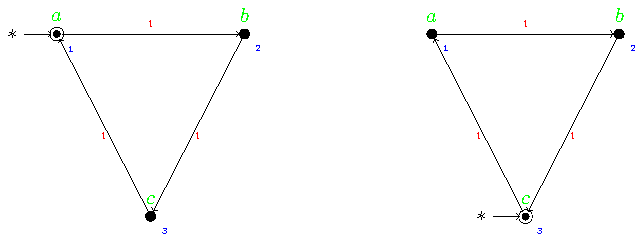
\includegraphics[scale=0.7]{images/counterexample.pdf}
%	\caption{Two TGs, $Q$ (left) and $R$ (right), having a different set of traces but the same embedding representation.}\label{fig:counterexample}
%\end{figure}
%\begin{example}
%	If we use $\epsilon$ (or $\epsilon^2$) and $\nu$ (or $\nu^2$) for $\gorgembed$, we might have a false positive for ``weak equality'' if $Q=(s,s,L,R,w)$ and $R=(s',s',L,R,w)$ are both cycle graphs with $s\neq s'$, $\textit{label}(s)\neq\textit{label}(s')$, $\textit{label}(s)\neq\tau$, and $\textit{label}(s')\neq\tau$. An intuitive example of such situation is presented in Figure \ref{fig:counterexample}: both graphs will have the same frequency for both subtraces and nodes, and therefore have the same  $\epsilon$ and $\nu$ by construction. By having different initial and accepting node with  different labels, we have $\mathcal{W}_0^{\aleph_0}(Q)=\Set{\textup{a(bca)}^n|n\in\mathbb{N}}$ and $\mathcal{W}_0^{\aleph_0}(R)=\Set{\textup{c(abc)}^n|n\in\mathbb{N}}$, thus implying $\mathcal{W}_0^{\aleph_0}(Q)\neq\mathcal{W}_0^{\aleph_0}(R)$ but $k_{\gorgembed}(Q,R)=1$ for $t_f=1$.
%\end{example}
%
%
%\begin{lemma}[Weak Equality]
%	Given two TGs $P=(s,t,L,R,w)$ and $P'=(s',t',L',R',w')$ providing the same set of weighted traces, then $k_{\gorgembed}(P,P')=ww'$ for $t_f=1$.
%\end{lemma}
%%\begin{proof}
%%	\xout{Given Proposition \ref{lem:rewritinglemma} and the positive definition of $\epsilon$ and $\nu$,  we have that $\norm{\hat{\epsilon}-\hat{\epsilon}'}{2}\to 0$ as well as $\norm{\hat{\nu}-\hat{\nu}'}{2}\to 0$, for which we can immediately close the goal.}
%%\end{proof}
%
%%\xout{As per previous observations, we know that}
%Two TGs should have the maximum dissimilarity when all the non $\tau$-nodes have different labels, thus making it impossible to find an alignment, thus implying that they share an utterly dissimilar set of weighted traces:
%
%\begin{lemma}[Strong Dissimilarity]
%	Given two TGs $P=(s,t,L,R,w)$ and $P'=(s',t',L',R',w')$, $k_{\gorgembed}(P,P')=0$ iff. $P$ and $P'$ have a different set of labels with $t_f,w,w'>0$.
%\end{lemma}
%%\begin{proof}
%%	\xout{If we exclude the trivial conditions $t_f=0$, $w=0$ or $w'=0$, the only condition when the kernel returns zero is when  $\Braket{\hat{\epsilon},\hat{\epsilon}'}=0$ and $\Braket{\hat{\nu},\hat{\nu}'}=0$. This implies that, when a component of $\epsilon$ (or $\nu$) is non-zero, the same component of $\epsilon'$ (or $\nu'$) is zero and viceversa. This directly requires that there is a different set of labels associated to the nodes. }
%%\end{proof}
%
%As a corollary of the two lemmas, we have that the proposed embedding performs weakly-ideally as defined in \S\ref{subsec:katk}, as equality condition holds in a relaxed form.
%
%Last, under the assumption that a TG is approximately characterized by $\epsilon$ and $\nu$, we might expect that the TG similarity is characterized by the sum of the distance of both embeddings. Therefore, we show that an increase in both distance embeddings approximately corresponds to a decrease in the kernel output and vice-versa.
%
%\begin{lemma}\label{lem:approxRank}
%	Given two TGs $P=(s,t,L,R,w)$ and $P'=(s',t',L',R',w')$ having respectively the embeddings $(\epsilon,\nu)$ and $(\epsilon',\nu')$, we have that the kernel $k_{\trembed}$ induces an inverse ranking of $\norm{\hat{\epsilon}-\hat{\epsilon}'}{2}+\norm{\hat{\nu}-\hat{\nu}'}{2}$:
%	$$k_{\trembed}(P,P')\appropto 2-(\norm{\hat{\epsilon}-\hat{\epsilon}'}{2}+\norm{\hat{\nu}-\hat{\nu}'}{2})$$
%\end{lemma}
%%\begin{proof}
%%	\xout{Let us use $T=t_f^{|R>0|+|R'>0|}$, $\omega=ww'$, $V=\norm{\hat{\nu}-\hat{\nu}'}{2}$, and $E=\norm{\hat{\epsilon}-\hat{\epsilon}'}{2}$ as shorthands. The goal can be rewritten as $k_{\trembed}(P,P')\appropto 2-(E+V)$. Given that the embeddings $(\epsilon,\nu)$ and $(\epsilon',\nu')$ are normalized kernel function $k_{\gorgembed}$ and that they are always positive definite, then we have that $0\leq E +V\leq 2$, so $0\leq 2-(E+V)\leq 2$. Using Proposition \ref{lem:rewritinglemma}, we can write $k_{\gorgembed}(P,P')$ as follows:}
%%	$$\Rcancel{\left(1-\frac{E}{2}\right)\omega T+\left(1-\frac{V}{2}\right)T=T\left(\omega+1-\frac{E\omega+V}{2}\right)}$$
%%	\xout{Given that the embeddings $(\epsilon,\nu)$ and $(\epsilon',\nu')$ are normalized in $k$ and that they are always positive definite,  we also have that $0\leq E\omega +V\leq 2$ where $0\leq \omega\leq 1$. We can also write  $0\leq \omega+1-\frac{E\omega+V}{2}\leq \frac{2}{T}$. For $\omega,T=1$, we have that $k_{\gorgembed}(P,P')=2-\frac{(E+V)}{2}$. Thus, $0<\omega,T<1$ approximates the expected ranking. }
%%\end{proof}
%
%%\ADD{Such lemma is going to be empirically evaluated in our experiment section.}

\subsubsection*{Acknowledgments}
This research has been partially supported by the project IDEE (FESR1133) funded by the Eur.\ Reg.\ Development Fund (ERDF) Investment for Growth and Jobs Programme 2014-2020.

\begin{table}[!t]
\caption{Distinct USWNs and associated sets of unravelled traces from a single Sepsis Cases Event Log \cite{mannhardt_2016}.}\label{tab:dataset}
 \begin{adjustbox}{max width=\textwidth}
	\begin{tabular}{crl||cl|c}
		\toprule
		\textbf{Experiment Conf.} $(\mathcal{U})$ & \textit{Model} & $+$\textit{W. Estimator} & $n$ & $p_\theta$& $\;\;|\mathcal{W}_{p_\theta}^n(P_{\mathcal{U}})|$ \\
		\midrule
		
		\textbf{SM\_CONS\_20} &SplitMiner 2.0  \cite{AugustoCDRP19}       & +\texttt{Constant} & $20$ & $\;\;0$ & $157$  \\
		
		\textbf{SM\_FORK\_20} & SplitMiner 2.0  \cite{AugustoCDRP19}      & +Fork \cite{spdwe} & $20$ & $\;\;0$ & $32$  \\
		
		
		\textbf{SM\_PAIR\_20} & SplitMiner 2.0  \cite{AugustoCDRP19}      & +PairScale \cite{spdwe} & $20$ & $\;\;0$ & $157$ \\
		
		\textbf{SM\_PETRI\_20} & \multicolumn{2}{c||}{Rogge-Solti \cite{RoggeSoltiAW13}} & $20$ & $10^{-5}$ & $1612$ \\
		\bottomrule
	\end{tabular}
\end{adjustbox}
\end{table}
\section{Experimental Results}\label{sec:exp}
\subsection{Dataset}
For our experiments, we took the Sepsis Cases Event Log \cite{mannhardt_2016}, splitted the dataset into the ``\textit{happy traces}'' occurring approximately near to the trace average length ($\leq 2.3\cdot 10^{7}$ ms), and used this dataset to generate either a USWN via ProM \cite{RoggeSoltiAW13} and a BPMN with only exclusive gates using Split Miner 2.0 \cite{AugustoCDRP19} that was then converted into a Petri Net \cite{PPNFromLog}. Such Petri Net was later on converted into a USWN by using a firing weight estimator: we choose the Fork and the PairScale estimators from \cite{spdwe} and we denote as \texttt{Constant} a naïve estimator assuming that each all the transition probabilities from a given marking are equiprobable. No estimator was used for the USWN generated via ProM, as such engine already estimates the firing weights. From such USWNs, we generate distinct sets of unravelled traces. All these steps are summarised in Table \ref{tab:dataset}. The following experiments have the aim of evaluating the benefits of performing the Approximate-Ranking strategy over the Optimal-Ranking one.

\begin{figure*}[!t]
\begin{minipage}{.49\textwidth}

	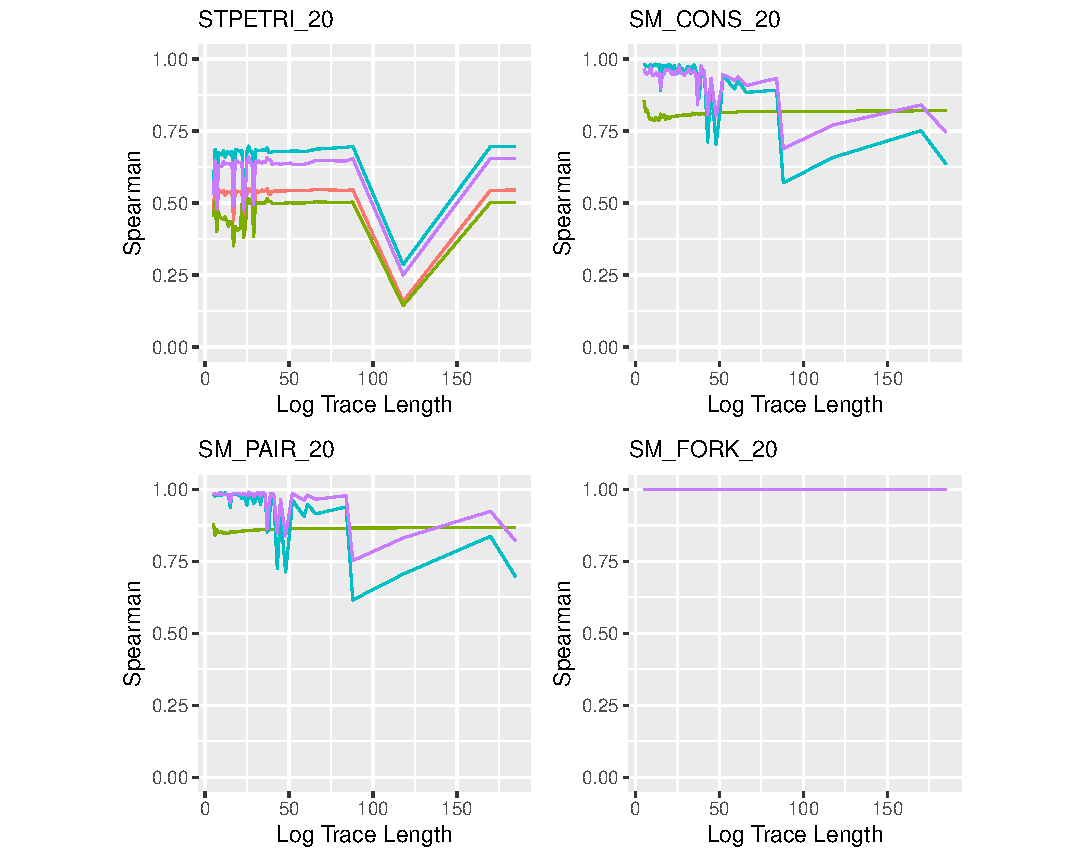
\includegraphics[width=1.1\textwidth]{images/Prec.pdf}
	\caption{Approximation comparison.}\label{fig:app}
\end{minipage}\hfill \begin{minipage}{.49\textwidth}

	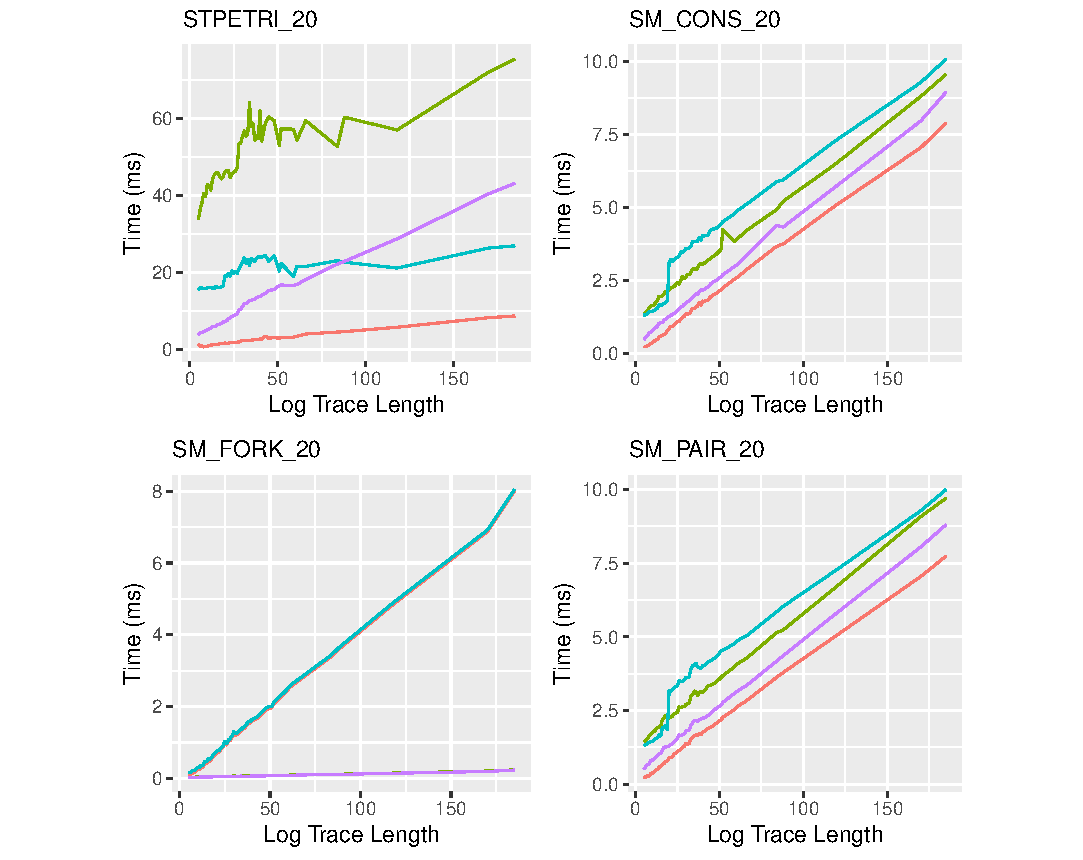
\includegraphics[width=1.1\textwidth]{images/kronos.pdf}
	\caption{$k$NN alignment benchmark.}\label{fig:kronos}
\end{minipage}
\end{figure*}
\subsection{Approximation}\label{subsec:apprp}
In order to assess how well the proposed Approximate-Ranking strategy approximates the Optimal-Ranking one, we use the Spearman Correlation Index \cite{} to express the correlation between each sub-embedding strategies for $\phi_{\mathcal{P}}$ ($\color{ggplotGreen}\epsilon^1\&\nu^1$, $\color{ggplotRed}\epsilon^2\&\nu^1$, $\color{ggplotPurple}\epsilon^1\&\nu^2$, and $\color{ggplotBlue}\epsilon^2\&\nu^2$) and the Optimal-Ranking one.
In general, we can see form the plots that when aligning longer traces, the correlation of the approximate rankings with the optimal one is lower. This is due to the fact that, in this case, the embedding representing the trace to align is longer and this implies also a larger approximation error. We can also observe that the sub-embeddings considering only information about the edges (i.e., the one where the features corresponding to the $\nu$ dimension are set to zero) have in general a higher correlation with the Optimal-Ranking strategy, but their correlation values are less stable with respect to the length of the trace to be aligned. In the case of \textbf{SM\_FORK\_20}, the correlation is maximum for all sub-embedding strategies.

%set of unravelled traces in Table \ref{tab:dataset} and the subset of the Sepsis Cases Event Log that was not used to generate the USWNs. For each of this log trace $\sigma^*$ we added controlled noise (transition addition, deletion, or swap) at either $20\%$ ($\tilde{\sigma}^*$) or $30\%$ ($\tilde{\tilde{{\sigma}}}^*$) of the log trace as for \cite{LeoniM17}. Then, we found the correlation between the ranking $R_\star$ induced by $k_{\phi_{\mathcal{P}}}(\sigma,\sigma^*)$ to the ranking induced by replacing $\sigma^*$ with one of the two noised traces (either a ranking $R_{20}$ induced by $k_{\phi_{\mathcal{P}}}(\sigma,\tilde{\sigma}^*)$ or $R_{30}$ induced by $k_{\phi_{\mathcal{P}}}(\sigma,\tilde{\tilde{\sigma}}^*)$). The correlation $\rho$ between these two rankings ($\rho(R_\star,R_{20})$ and $\rho(R_\star,R_{30})$) is performed via Spearman Correlation Index $\rho$: such index will return near-$1$ on increasing monotonic trend, near-$(-1)$ values on decreasing monotonic trend, and near-$0$ values where the two rankings are almost uncorrelated. Figure \ref{fig:app} shows the outcome of such experiments for all the possible combinations of $\epsilon$ and $\nu$ sub-embeddings for $\phi_{\mathcal{P}}$ while varying the log trace length. We can observe that strategies including traces' frequencies ($\nu^1$) are more stable if compared to strategies where such information is completely ignored ($\nu^2$). Furthermore, such approximation never reaches zero values, while that occurrence might happen for $\nu^2$-based strategies.

\subsection{Efficiency}\label{subsec:efficio}
With reference to the plots in Figure \ref{fig:kronos}, 
we evaluated the efficiency of computing the trace alignment over both Optimal- ({\color{ggplotPurple}Purple} and {\color{ggplotGreen}Green}) and Approximated-ranking ({\color{ggplotBlue}Blue} and {\color{ggplotRed}Red}) strategies over two different data structures enabling $k$NN queries, i.e., VP-Trees ({\color{ggplotBlue}Blue} and {\color{ggplotPurple}Purple}) and KD-Trees ({\color{ggplotRed}Red} and {\color{ggplotGreen}Green}). We conduct our experiments for $k=20$\ADD{, and we use the Levenshtein distance as a baseline distance for the alignment cost function}. While the query time for the Optimal-Ranking  includes the additional \textit{indexing time} for generating all the vectors to the neighbourhood search, the Approximated-Ranking  adds the neighbourhood search time with the embedding transformation of $x$; in particular, we consider the average embedding time for all the possible embedding strategies described in the previous experiment setting. Figure \ref{fig:kronos} plots the result of such experiments: the time required to generate and load all the $\phi_\star$ truly dominates the cost of generating the embedding $\phi_{\mathcal{P}}(x)$ for bigger datasets such as \textbf{STPETRI\_20}, while the cost for $\phi_{\mathcal{P}}(x)$ becomes non-negligible when we have just a few traces to align (\textbf{SM\_FORK\_20}). Last, while the $k$NN alignments over $\phi_{\mathcal{P}}$ always provide the best timing results via KD-Trees, we cannot elect a best data structure $\phi_\star$ that is valid for all datasets and all trace lengths. 
%\section{Conclusions}
%\texttt{\color{red}[TODO]}
%\label{sec:conclusion}
%
%We have studied how to enrich constraint-based process models with uncertainty, captured as the probability that a trace will conform with a constraint or not. We have discussed how this impacts the semantics of a constraint model, and how logical and probabilistic reasoning have to be combined to provide core services such as consistency and conformance checking, as well as probabilistic constraint entailment.
%
%Notably, all the techniques presented in this paper can be directly grounded with existing tools: automata-based techniques for \LTLf to carry out logical reasoning, and off-the-shelf systems to solve systems of linear inequalities (and corresponding optimization problems) to handle probabilities.
%
%In~\cite{DBLP:conf/bpm/Maggi2020}, beside a concrete implementation of the techniques presented in this paper, we investigate the application of probabilistic business constraints to process mining, not only considering standard problems like discovery, but also delving into online operational support and, in particular, probabilistic monitoring~\cite{DBLP:conf/fase/MaggiMA12}.

%Balancing between the likelihood of the model trace with respect to which we are computing the alignment and the cost of the alignment (if the cost of the alignment is too high even if the model trace is very likely applying too many changes in the original trace is in turn not very likely).

%\section*{Acknowledgements}


%This research has been partially supported by the project IDEE (FESR1133) funded by the Eur.\ Reg.\ Development Fund (ERDF) Investment for Growth and Jobs Programme 2014-2020. 


\bibliographystyle{splncs04}
\bibliography{biblio3}
%,bibliography2,references,libraryFiltered,main,Bibliography-CDC,DiCiccio,biblio}


%\bibliographystyle{stylename}
%\bibliography{bibfile}


\end{document}
